\documentclass[twoside]{book}

% Packages required by doxygen
\usepackage{calc}
\usepackage{doxygen}
\usepackage{graphicx}
\usepackage[utf8]{inputenc}
\usepackage{makeidx}
\usepackage{multicol}
\usepackage{multirow}
\usepackage{textcomp}
\usepackage[table]{xcolor}

% Font selection
\usepackage[T1]{fontenc}
\usepackage{mathptmx}
\usepackage[scaled=.90]{helvet}
\usepackage{courier}
\usepackage{amssymb}
\usepackage{sectsty}
\renewcommand{\familydefault}{\sfdefault}
\allsectionsfont{%
  \fontseries{bc}\selectfont%
  \color{darkgray}%
}
\renewcommand{\DoxyLabelFont}{%
  \fontseries{bc}\selectfont%
  \color{darkgray}%
}

% Page & text layout
\usepackage{geometry}
\geometry{%
  a4paper,%
  top=2.5cm,%
  bottom=2.5cm,%
  left=2.5cm,%
  right=2.5cm%
}
\tolerance=750
\hfuzz=15pt
\hbadness=750
\setlength{\emergencystretch}{15pt}
\setlength{\parindent}{0cm}
\setlength{\parskip}{0.2cm}
\makeatletter
\renewcommand{\paragraph}{%
  \@startsection{paragraph}{4}{0ex}{-1.0ex}{1.0ex}{%
    \normalfont\normalsize\bfseries\SS@parafont%
  }%
}
\renewcommand{\subparagraph}{%
  \@startsection{subparagraph}{5}{0ex}{-1.0ex}{1.0ex}{%
    \normalfont\normalsize\bfseries\SS@subparafont%
  }%
}
\makeatother

% Headers & footers
\usepackage{fancyhdr}
\pagestyle{fancyplain}
\fancyhead[LE]{\fancyplain{}{\bfseries\thepage}}
\fancyhead[CE]{\fancyplain{}{}}
\fancyhead[RE]{\fancyplain{}{\bfseries\leftmark}}
\fancyhead[LO]{\fancyplain{}{\bfseries\rightmark}}
\fancyhead[CO]{\fancyplain{}{}}
\fancyhead[RO]{\fancyplain{}{\bfseries\thepage}}
\fancyfoot[LE]{\fancyplain{}{}}
\fancyfoot[CE]{\fancyplain{}{}}
\fancyfoot[RE]{\fancyplain{}{\bfseries\scriptsize Generated on Mon May 30 2016 12\-:37\-:21 for Multiphase Flow by Doxygen }}
\fancyfoot[LO]{\fancyplain{}{\bfseries\scriptsize Generated on Mon May 30 2016 12\-:37\-:21 for Multiphase Flow by Doxygen }}
\fancyfoot[CO]{\fancyplain{}{}}
\fancyfoot[RO]{\fancyplain{}{}}
\renewcommand{\footrulewidth}{0.4pt}
\renewcommand{\chaptermark}[1]{%
  \markboth{#1}{}%
}
\renewcommand{\sectionmark}[1]{%
  \markright{\thesection\ #1}%
}

% Indices & bibliography
\usepackage{natbib}
\usepackage[titles]{tocloft}
\setcounter{tocdepth}{3}
\setcounter{secnumdepth}{5}
\makeindex

% Hyperlinks (required, but should be loaded last)
\usepackage{ifpdf}
\ifpdf
  \usepackage[pdftex,pagebackref=true]{hyperref}
\else
  \usepackage[ps2pdf,pagebackref=true]{hyperref}
\fi
\hypersetup{%
  colorlinks=true,%
  linkcolor=blue,%
  citecolor=blue,%
  unicode%
}

% Custom commands
\newcommand{\clearemptydoublepage}{%
  \newpage{\pagestyle{empty}\cleardoublepage}%
}


%===== C O N T E N T S =====

\begin{document}

% Titlepage & ToC
\hypersetup{pageanchor=false}
\pagenumbering{roman}
\begin{titlepage}
\vspace*{7cm}
\begin{center}%
{\Large Multiphase Flow }\\
\vspace*{1cm}
{\large Generated by Doxygen 1.8.5}\\
\vspace*{0.5cm}
{\small Mon May 30 2016 12:37:21}\\
\end{center}
\end{titlepage}
\clearemptydoublepage
\tableofcontents
\clearemptydoublepage
\pagenumbering{arabic}
\hypersetup{pageanchor=true}

%--- Begin generated contents ---
\chapter{Hierarchical Index}
\section{Class Hierarchy}
This inheritance list is sorted roughly, but not completely, alphabetically\-:\begin{DoxyCompactList}
\item \contentsline{section}{Computation}{\pageref{classComputation}}{}
\item \contentsline{section}{Constants}{\pageref{classConstants}}{}
\item \contentsline{section}{F\-O\-R\-C\-E}{\pageref{classFORCE}}{}
\item \contentsline{section}{Grid}{\pageref{classGrid}}{}
\item \contentsline{section}{Konstanten}{\pageref{classKonstanten}}{}
\item \contentsline{section}{Numerical\-\_\-\-Method}{\pageref{classNumerical__Method}}{}
\item \contentsline{section}{Solver}{\pageref{classSolver}}{}
\begin{DoxyCompactList}
\item \contentsline{section}{Force}{\pageref{classForce}}{}
\item \contentsline{section}{Lax\-\_\-\-Friedrich}{\pageref{classLax__Friedrich}}{}
\end{DoxyCompactList}
\end{DoxyCompactList}

\chapter{Class Index}
\section{Class List}
Here are the classes, structs, unions and interfaces with brief descriptions\-:\begin{DoxyCompactList}
\item\contentsline{section}{\hyperlink{classComputation}{Computation} }{\pageref{classComputation}}{}
\item\contentsline{section}{\hyperlink{classConstants}{Constants} }{\pageref{classConstants}}{}
\item\contentsline{section}{\hyperlink{classFORCE}{F\-O\-R\-C\-E} }{\pageref{classFORCE}}{}
\item\contentsline{section}{\hyperlink{classForce}{Force} }{\pageref{classForce}}{}
\item\contentsline{section}{\hyperlink{classGrid}{Grid} }{\pageref{classGrid}}{}
\item\contentsline{section}{\hyperlink{classKonstanten}{Konstanten} }{\pageref{classKonstanten}}{}
\item\contentsline{section}{\hyperlink{classLax__Friedrich}{Lax\-\_\-\-Friedrich} }{\pageref{classLax__Friedrich}}{}
\item\contentsline{section}{\hyperlink{classNumerical__Method}{Numerical\-\_\-\-Method} }{\pageref{classNumerical__Method}}{}
\item\contentsline{section}{\hyperlink{classSolver}{Solver} }{\pageref{classSolver}}{}
\end{DoxyCompactList}

\chapter{Class Documentation}
\hypertarget{classComputation}{\section{Computation Class Reference}
\label{classComputation}\index{Computation@{Computation}}
}


{\ttfamily \#include $<$computation.\-h$>$}

\subsection*{Public Member Functions}
\begin{DoxyCompactItemize}
\item 
void \hyperlink{classComputation_af2a835928bcf124b803756730b47aecb}{compute\-\_\-u\-\_\-1d} (double $\ast$$\ast$$\ast$u, \hyperlink{classGrid}{Grid} $\ast$grid)
\item 
void \hyperlink{classComputation_a6ae111f850757aa9e494b25fa397bfb5}{compute\-\_\-f\-\_\-1d} (double $\ast$$\ast$$\ast$f, \hyperlink{classGrid}{Grid} $\ast$grid)
\item 
void \hyperlink{classComputation_a158cbdbd7b5a770b9e96175287421dd1}{compute\-\_\-u\-\_\-2d} (double $\ast$$\ast$$\ast$u, \hyperlink{classGrid}{Grid} $\ast$grid)
\item 
void \hyperlink{classComputation_a86cd911682059748fa6a0031c69275f0}{compute\-\_\-f\-\_\-2d} (double $\ast$$\ast$$\ast$f, \hyperlink{classGrid}{Grid} $\ast$grid)
\item 
void \hyperlink{classComputation_aa41d173cd841966f00bedd9e040b5e78}{compute\-\_\-g\-\_\-2d} (double $\ast$$\ast$$\ast$g, \hyperlink{classGrid}{Grid} $\ast$grid)
\end{DoxyCompactItemize}
\subsection*{Static Public Member Functions}
\begin{DoxyCompactItemize}
\item 
\hypertarget{classComputation_a8900cb37bdf5e88b60c3472423df8bbf}{static \hyperlink{classComputation}{Computation} \& {\bfseries instance} (\hyperlink{classConstants}{Constants} $\ast$\hyperlink{classComputation_ad83b15fa4885674df22b99bb3f9ffc40}{constants})}\label{classComputation_a8900cb37bdf5e88b60c3472423df8bbf}

\end{DoxyCompactItemize}
\subsection*{Public Attributes}
\begin{DoxyCompactItemize}
\item 
int \hyperlink{classComputation_a927cc1ebb3cadf7a465eb8cd1144beed}{neqs}
\item 
\hyperlink{classConstants}{Constants} $\ast$ \hyperlink{classComputation_ad83b15fa4885674df22b99bb3f9ffc40}{constants}
\item 
\hypertarget{classComputation_a5f3502842df5af2e1303bc147aea89d7}{double {\bfseries cref}}\label{classComputation_a5f3502842df5af2e1303bc147aea89d7}

\item 
\hypertarget{classComputation_ab232a054e34ed21bfa7a24f833c93b57}{double {\bfseries done}}\label{classComputation_ab232a054e34ed21bfa7a24f833c93b57}

\item 
\hypertarget{classComputation_af9e1a00de0bc1d24ecb5af19c5353d12}{double {\bfseries ccl}}\label{classComputation_af9e1a00de0bc1d24ecb5af19c5353d12}

\item 
\hypertarget{classComputation_a3c28d827c509596982f121cb59338361}{double {\bfseries gamma}}\label{classComputation_a3c28d827c509596982f121cb59338361}

\item 
\hypertarget{classComputation_a74b3040ac82fbffe2c6fe90920a86b86}{double {\bfseries ccl12}}\label{classComputation_a74b3040ac82fbffe2c6fe90920a86b86}

\item 
\hypertarget{classComputation_aaebd39f609368178f1ac5a144c24a49f}{double {\bfseries ccl12h}}\label{classComputation_aaebd39f609368178f1ac5a144c24a49f}

\item 
\hypertarget{classComputation_ac4c32bee51db9e26193a68843e739397}{double {\bfseries gcinv}}\label{classComputation_ac4c32bee51db9e26193a68843e739397}

\item 
\hypertarget{classComputation_aae3ea92e493ef3b703e8c21fa9eaf24e}{double {\bfseries gcdgcm1}}\label{classComputation_aae3ea92e493ef3b703e8c21fa9eaf24e}

\item 
\hypertarget{classComputation_ad3fb5d8835f9dfddc6c8c56b491abe0e}{double {\bfseries gcm1dgc}}\label{classComputation_ad3fb5d8835f9dfddc6c8c56b491abe0e}

\item 
\hypertarget{classComputation_a4e063ea6fb7dc463b28eda000a837fe7}{double {\bfseries cclm1}}\label{classComputation_a4e063ea6fb7dc463b28eda000a837fe7}

\item 
\hypertarget{classComputation_a1fade3b3ea69fb28256f5cb6eb453333}{double {\bfseries powcref}}\label{classComputation_a1fade3b3ea69fb28256f5cb6eb453333}

\end{DoxyCompactItemize}


\subsection{Detailed Description}
Die Klasse \hyperlink{classComputation}{Computation} verwaltet die Formelvektoren u,f\-\_\-u und s\-\_\-u. Die Formelvektoren wurden in der ursprüngliche Version als Strings in Vektoren abgespeichert, und dann mittels Funktionen der exprtk Libiary interpretiert, aber das dauerte viel zu lange 

\subsection{Member Function Documentation}
\hypertarget{classComputation_a6ae111f850757aa9e494b25fa397bfb5}{\index{Computation@{Computation}!compute\-\_\-f\-\_\-1d@{compute\-\_\-f\-\_\-1d}}
\index{compute\-\_\-f\-\_\-1d@{compute\-\_\-f\-\_\-1d}!Computation@{Computation}}
\subsubsection[{compute\-\_\-f\-\_\-1d}]{\setlength{\rightskip}{0pt plus 5cm}void Computation\-::compute\-\_\-f\-\_\-1d (
\begin{DoxyParamCaption}
\item[{double $\ast$$\ast$$\ast$}]{f, }
\item[{{\bf Grid} $\ast$}]{grid}
\end{DoxyParamCaption}
)}}\label{classComputation_a6ae111f850757aa9e494b25fa397bfb5}
Berechnet die Lösungen der Formel für den Fluss F in 1-\/\-D 
\begin{DoxyParams}{Parameters}
{\em f,3-\/d} & Feld für die F-\/\-Werte \\
\hline
{\em Raster,welche} & die Werte zur Berechnung enthält. \\
\hline
{\em cells,Ausdehnung} & des Gitters \\
\hline
{\em ordnung} & des Algorithmus, wichtig für die Ausdehnung des Gitters \\
\hline
\end{DoxyParams}
\hypertarget{classComputation_a86cd911682059748fa6a0031c69275f0}{\index{Computation@{Computation}!compute\-\_\-f\-\_\-2d@{compute\-\_\-f\-\_\-2d}}
\index{compute\-\_\-f\-\_\-2d@{compute\-\_\-f\-\_\-2d}!Computation@{Computation}}
\subsubsection[{compute\-\_\-f\-\_\-2d}]{\setlength{\rightskip}{0pt plus 5cm}void Computation\-::compute\-\_\-f\-\_\-2d (
\begin{DoxyParamCaption}
\item[{double $\ast$$\ast$$\ast$}]{f, }
\item[{{\bf Grid} $\ast$}]{grid}
\end{DoxyParamCaption}
)}}\label{classComputation_a86cd911682059748fa6a0031c69275f0}
Berechnet die Lösungen der Formel für den Fluss F in 2-\/\-D 
\begin{DoxyParams}{Parameters}
{\em f,3-\/d} & Feld für die F-\/\-Werte \\
\hline
{\em Raster,welche} & die Werte zur Berechnung enthält. \\
\hline
{\em cells,Ausdehnung} & des Gitters \\
\hline
{\em ordnung} & des Algorithmus, wichtig für die Ausdehnung des Gitters \\
\hline
\end{DoxyParams}
\hypertarget{classComputation_aa41d173cd841966f00bedd9e040b5e78}{\index{Computation@{Computation}!compute\-\_\-g\-\_\-2d@{compute\-\_\-g\-\_\-2d}}
\index{compute\-\_\-g\-\_\-2d@{compute\-\_\-g\-\_\-2d}!Computation@{Computation}}
\subsubsection[{compute\-\_\-g\-\_\-2d}]{\setlength{\rightskip}{0pt plus 5cm}void Computation\-::compute\-\_\-g\-\_\-2d (
\begin{DoxyParamCaption}
\item[{double $\ast$$\ast$$\ast$}]{g, }
\item[{{\bf Grid} $\ast$}]{grid}
\end{DoxyParamCaption}
)}}\label{classComputation_aa41d173cd841966f00bedd9e040b5e78}
Berechnet die Lösungen der Formel für den Fluss G in 2-\/\-D 
\begin{DoxyParams}{Parameters}
{\em Raster,welche} & die Werte zur Berechnung enthält. \\
\hline
{\em cells,Ausdehnung} & des Gitters \\
\hline
{\em ordnung} & des Algorithmus, wichtig für die Ausdehnung des Gitters\\
\hline
\end{DoxyParams}
Berechnet die Lösungen der Formel für den Fluss G in 2-\/\-D 
\begin{DoxyParams}{Parameters}
{\em g,3-\/d} & Feld für die G-\/\-Werte \\
\hline
{\em Raster,welche} & die Werte zur Berechnung enthält. \\
\hline
{\em cells,Ausdehnung} & des Gitters \\
\hline
{\em ordnung} & des Algorithmus, wichtig für die Ausdehnung des Gitters \\
\hline
\end{DoxyParams}
\hypertarget{classComputation_af2a835928bcf124b803756730b47aecb}{\index{Computation@{Computation}!compute\-\_\-u\-\_\-1d@{compute\-\_\-u\-\_\-1d}}
\index{compute\-\_\-u\-\_\-1d@{compute\-\_\-u\-\_\-1d}!Computation@{Computation}}
\subsubsection[{compute\-\_\-u\-\_\-1d}]{\setlength{\rightskip}{0pt plus 5cm}void Computation\-::compute\-\_\-u\-\_\-1d (
\begin{DoxyParamCaption}
\item[{double $\ast$$\ast$$\ast$}]{u, }
\item[{{\bf Grid} $\ast$}]{grid}
\end{DoxyParamCaption}
)}}\label{classComputation_af2a835928bcf124b803756730b47aecb}
Vektor von u Rückrechnung der erhaltenen Variablen in die physikalischen. Vektor der Formeln von f\-\_\-u. Vektor der Formeln von g\-\_\-u. Berechnet die Werte U in 1-\/\-D 
\begin{DoxyParams}{Parameters}
{\em u,3-\/d} & Feld für die U-\/\-Werte \\
\hline
{\em Raster,welche} & die Werte zur Berechnung enthält. \\
\hline
{\em cells,Ausdehnung} & des Gitters \\
\hline
{\em ordnung} & des Algorithmus, wichtig für die Ausdehnung des Gitters\\
\hline
\end{DoxyParams}
Berechnet die Werte U in 1-\/\-D 
\begin{DoxyParams}{Parameters}
{\em u,3-\/d} & Feld für die U-\/\-Werte \\
\hline
{\em raster,welche} & die Werte zur Berechnung enthält. \\
\hline
{\em cells,Ausdehnung} & des Gitters \\
\hline
{\em ordnung} & des Algorithmus, wichtig für die Ausdehnung des Gitters \\
\hline
\end{DoxyParams}
\hypertarget{classComputation_a158cbdbd7b5a770b9e96175287421dd1}{\index{Computation@{Computation}!compute\-\_\-u\-\_\-2d@{compute\-\_\-u\-\_\-2d}}
\index{compute\-\_\-u\-\_\-2d@{compute\-\_\-u\-\_\-2d}!Computation@{Computation}}
\subsubsection[{compute\-\_\-u\-\_\-2d}]{\setlength{\rightskip}{0pt plus 5cm}void Computation\-::compute\-\_\-u\-\_\-2d (
\begin{DoxyParamCaption}
\item[{double $\ast$$\ast$$\ast$}]{u, }
\item[{{\bf Grid} $\ast$}]{grid}
\end{DoxyParamCaption}
)}}\label{classComputation_a158cbdbd7b5a770b9e96175287421dd1}
Berechnet die Werte U in 2-\/\-D 
\begin{DoxyParams}{Parameters}
{\em u,3-\/d} & Feld für die U-\/\-Werte \\
\hline
{\em Raster,welche} & die Werte zur Berechnung enthält. \\
\hline
{\em cells,Ausdehnung} & des Gitters \\
\hline
{\em ordnung} & des Algorithmus, wichtig für die Ausdehnung des Gitters \\
\hline
\end{DoxyParams}


\subsection{Member Data Documentation}
\hypertarget{classComputation_ad83b15fa4885674df22b99bb3f9ffc40}{\index{Computation@{Computation}!constants@{constants}}
\index{constants@{constants}!Computation@{Computation}}
\subsubsection[{constants}]{\setlength{\rightskip}{0pt plus 5cm}{\bf Constants}$\ast$ Computation\-::constants}}\label{classComputation_ad83b15fa4885674df22b99bb3f9ffc40}
Abgespeichertes \hyperlink{classKonstanten}{Konstanten} Objekt. Wird nur einmal beim Konstruktor gesetzt, damit es bei Rechnungen nicht immer neu übergeben werden muss. \hypertarget{classComputation_a927cc1ebb3cadf7a465eb8cd1144beed}{\index{Computation@{Computation}!neqs@{neqs}}
\index{neqs@{neqs}!Computation@{Computation}}
\subsubsection[{neqs}]{\setlength{\rightskip}{0pt plus 5cm}int Computation\-::neqs}}\label{classComputation_a927cc1ebb3cadf7a465eb8cd1144beed}
Anzahl der Gleichungen 

The documentation for this class was generated from the following files\-:\begin{DoxyCompactItemize}
\item 
computation.\-h\item 
computation.\-cpp\end{DoxyCompactItemize}

\hypertarget{classConstants}{\section{Constants Class Reference}
\label{classConstants}\index{Constants@{Constants}}
}
\subsection*{Static Public Member Functions}
\begin{DoxyCompactItemize}
\item 
\hypertarget{classConstants_a1a022576d89b01d8706558e277739ca5}{static \hyperlink{classConstants}{Constants} \& {\bfseries instance} ()}\label{classConstants_a1a022576d89b01d8706558e277739ca5}

\end{DoxyCompactItemize}
\subsection*{Public Attributes}
\begin{DoxyCompactItemize}
\item 
std\-::string \hyperlink{classConstants_a6551e0c666c13d6c4fca96ee5585fa7c}{input\-\_\-const}
\item 
\hypertarget{classConstants_a8092bbe0ee648af855e48cb81da95439}{int {\bfseries calceigv}}\label{classConstants_a8092bbe0ee648af855e48cb81da95439}

\item 
\hypertarget{classConstants_ae254c67830baf0b06a041962c70506b0}{int {\bfseries variante}}\label{classConstants_ae254c67830baf0b06a041962c70506b0}

\item 
\hypertarget{classConstants_adf8539822dfaf47dfa490785bd272d08}{double {\bfseries teiler}}\label{classConstants_adf8539822dfaf47dfa490785bd272d08}

\item 
\hypertarget{classConstants_a3c97bfea56dd24e2d4bace4c8426a692}{int {\bfseries teilerend}}\label{classConstants_a3c97bfea56dd24e2d4bace4c8426a692}

\item 
\hypertarget{classConstants_a1e68104c2cf278844d1bb6f8443fc645}{double {\bfseries timeou}}\label{classConstants_a1e68104c2cf278844d1bb6f8443fc645}

\item 
\hypertarget{classConstants_a6a8cf48e105e96fd23bba4b151766687}{double {\bfseries cfl}}\label{classConstants_a6a8cf48e105e96fd23bba4b151766687}

\item 
\hypertarget{classConstants_a1b431477b01b2dd54ec23ff8cea4c4f4}{int {\bfseries maxnt}}\label{classConstants_a1b431477b01b2dd54ec23ff8cea4c4f4}

\item 
\hypertarget{classConstants_a9b4b7c840333c245bd654b265e828a39}{int {\bfseries dimension}}\label{classConstants_a9b4b7c840333c245bd654b265e828a39}

\item 
\hypertarget{classConstants_a3097ad771a07022e82bb873cf1027527}{int {\bfseries order}}\label{classConstants_a3097ad771a07022e82bb873cf1027527}

\item 
\hypertarget{classConstants_aeb97c511715fb70baeb5e26ea78afa32}{double {\bfseries radius}}\label{classConstants_aeb97c511715fb70baeb5e26ea78afa32}

\item 
\hypertarget{classConstants_a5d685a89ed3dbca064a4a905f5d54bbc}{int {\bfseries grid\-\_\-size\-\_\-x}}\label{classConstants_a5d685a89ed3dbca064a4a905f5d54bbc}

\item 
\hypertarget{classConstants_a694cb7e2a7c6677c321c6a680a3d57c8}{int {\bfseries grid\-\_\-size\-\_\-y}}\label{classConstants_a694cb7e2a7c6677c321c6a680a3d57c8}

\item 
\hypertarget{classConstants_a98be0914eaad9a6fc7e50df1aed6081d}{double {\bfseries gamma}}\label{classConstants_a98be0914eaad9a6fc7e50df1aed6081d}

\item 
\hypertarget{classConstants_ad170cfbcc36e2e559bb9ea406537d927}{double {\bfseries pos\-\_\-x\-\_\-min}}\label{classConstants_ad170cfbcc36e2e559bb9ea406537d927}

\item 
\hypertarget{classConstants_a9f1551700b1d5b347ed9aa370642bb8c}{double {\bfseries pos\-\_\-x\-\_\-max}}\label{classConstants_a9f1551700b1d5b347ed9aa370642bb8c}

\item 
\hypertarget{classConstants_a6dd6afa8e8c8b223ddbc9ff3e3bd4a2d}{double {\bfseries pos\-\_\-y\-\_\-min}}\label{classConstants_a6dd6afa8e8c8b223ddbc9ff3e3bd4a2d}

\item 
\hypertarget{classConstants_a936ebab57f6a62e0fba22be570e2367b}{double {\bfseries pos\-\_\-y\-\_\-max}}\label{classConstants_a936ebab57f6a62e0fba22be570e2367b}

\item 
\hypertarget{classConstants_ae3aa0d04a9b127b7e3c3a0eb5e4d09b5}{int {\bfseries bc\-\_\-y\-\_\-max}}\label{classConstants_ae3aa0d04a9b127b7e3c3a0eb5e4d09b5}

\item 
\hypertarget{classConstants_ae3ea4ac7704fa58c0668508018db88f4}{int {\bfseries bc\-\_\-y\-\_\-min}}\label{classConstants_ae3ea4ac7704fa58c0668508018db88f4}

\item 
\hypertarget{classConstants_a75a11e77f7983ed3be0ad18d0aebcead}{int {\bfseries bc\-\_\-x\-\_\-min}}\label{classConstants_a75a11e77f7983ed3be0ad18d0aebcead}

\item 
\hypertarget{classConstants_a55cc315b40e29df7b697371c2c670708}{int {\bfseries bc\-\_\-x\-\_\-max}}\label{classConstants_a55cc315b40e29df7b697371c2c670708}

\item 
\hypertarget{classConstants_a77b6679dcd080391066411ee1d888631}{double {\bfseries cref}}\label{classConstants_a77b6679dcd080391066411ee1d888631}

\item 
\hypertarget{classConstants_ae5f5c7ab6d15d912175737b374809da6}{double {\bfseries rho\-\_\-one}}\label{classConstants_ae5f5c7ab6d15d912175737b374809da6}

\item 
\hypertarget{classConstants_a84ce95697de981f89e1c5a5dfdf7457f}{double {\bfseries ccl}}\label{classConstants_a84ce95697de981f89e1c5a5dfdf7457f}

\item 
\hypertarget{classConstants_ad131d2c8a54e216cb5edddea47e683f6}{double {\bfseries rhol}}\label{classConstants_ad131d2c8a54e216cb5edddea47e683f6}

\item 
\hypertarget{classConstants_aaee23bce903deafee29ef7bc92ff4291}{double {\bfseries vl}}\label{classConstants_aaee23bce903deafee29ef7bc92ff4291}

\item 
\hypertarget{classConstants_ad1456b641e922da7e6fbdb1b5fce74c7}{double {\bfseries vrl}}\label{classConstants_ad1456b641e922da7e6fbdb1b5fce74c7}

\item 
\hypertarget{classConstants_a439e77e20421247bdae078f067d4ce46}{double {\bfseries vyl}}\label{classConstants_a439e77e20421247bdae078f067d4ce46}

\item 
\hypertarget{classConstants_a1de09fc7346cd5f8ca44b0f18db6438c}{double {\bfseries vyrl}}\label{classConstants_a1de09fc7346cd5f8ca44b0f18db6438c}

\item 
\hypertarget{classConstants_a46e542b95ecf979189899f829cd0f699}{double {\bfseries rhor}}\label{classConstants_a46e542b95ecf979189899f829cd0f699}

\item 
\hypertarget{classConstants_a7fa65dc6054d48012e4ac0859cc00de1}{double {\bfseries vr}}\label{classConstants_a7fa65dc6054d48012e4ac0859cc00de1}

\item 
\hypertarget{classConstants_a5a5ab51973e5ad985af0abc7d5063e1b}{double {\bfseries vrr}}\label{classConstants_a5a5ab51973e5ad985af0abc7d5063e1b}

\item 
\hypertarget{classConstants_a705882af1e5cfed966a4d567e6c36dd4}{double {\bfseries vyr}}\label{classConstants_a705882af1e5cfed966a4d567e6c36dd4}

\item 
\hypertarget{classConstants_a776070b16072b84b16b1b356a5a0b1ed}{double {\bfseries vyrr}}\label{classConstants_a776070b16072b84b16b1b356a5a0b1ed}

\item 
double \hyperlink{classConstants_aefb49d707a69e32ab5c0abb04bef07e2}{ct}
\end{DoxyCompactItemize}


\subsection{Member Data Documentation}
\hypertarget{classConstants_aefb49d707a69e32ab5c0abb04bef07e2}{\index{Constants@{Constants}!ct@{ct}}
\index{ct@{ct}!Constants@{Constants}}
\subsubsection[{ct}]{\setlength{\rightskip}{0pt plus 5cm}double Constants\-::ct}}\label{classConstants_aefb49d707a69e32ab5c0abb04bef07e2}
K in den Formeln. \hypertarget{classConstants_a6551e0c666c13d6c4fca96ee5585fa7c}{\index{Constants@{Constants}!input\-\_\-const@{input\-\_\-const}}
\index{input\-\_\-const@{input\-\_\-const}!Constants@{Constants}}
\subsubsection[{input\-\_\-const}]{\setlength{\rightskip}{0pt plus 5cm}std\-::string Constants\-::input\-\_\-const}}\label{classConstants_a6551e0c666c13d6c4fca96ee5585fa7c}
Beizeichnungen der \hyperlink{classKonstanten}{Konstanten} in einem Vektor. Vektor von Werten der \hyperlink{classKonstanten}{Konstanten}. 

The documentation for this class was generated from the following files\-:\begin{DoxyCompactItemize}
\item 
constants.\-h\item 
constants.\-cpp\end{DoxyCompactItemize}

\hypertarget{classFORCE}{\section{F\-O\-R\-C\-E Class Reference}
\label{classFORCE}\index{F\-O\-R\-C\-E@{F\-O\-R\-C\-E}}
}


{\ttfamily \#include $<$F\-O\-R\-C\-E.\-h$>$}

Inheritance diagram for F\-O\-R\-C\-E\-:\begin{figure}[H]
\begin{center}
\leavevmode
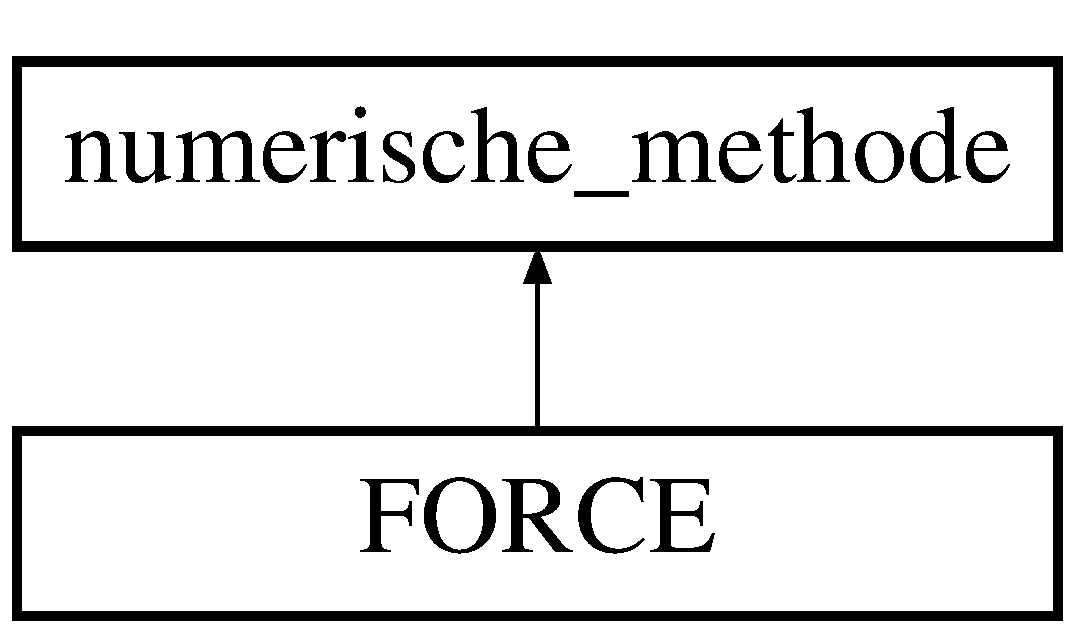
\includegraphics[height=2.000000cm]{classFORCE}
\end{center}
\end{figure}
\subsection*{Public Member Functions}
\begin{DoxyCompactItemize}
\item 
\hyperlink{classFORCE_a0dd4dcc9d89eb274f2f8ded4b3f48f89}{F\-O\-R\-C\-E} (std\-::string const\-\_\-in, std\-::string formel\-\_\-in, std\-::string save\-\_\-in)
\end{DoxyCompactItemize}
\subsection*{Protected Member Functions}
\begin{DoxyCompactItemize}
\item 
std\-::vector$<$ std\-::vector\\*
$<$ std\-::vector$<$ std\-::vector\\*
$<$ double $>$ $>$ $>$ $>$ \hyperlink{classFORCE_a03c0c50dc6e49e1d1b1f056cb76742e9}{calc\-\_\-method\-\_\-flux} (int dir)
\end{DoxyCompactItemize}
\subsection*{Additional Inherited Members}


\subsection{Detailed Description}
Klasse der \hyperlink{classFORCE}{F\-O\-R\-C\-E} Methode. 

\subsection{Constructor \& Destructor Documentation}
\hypertarget{classFORCE_a0dd4dcc9d89eb274f2f8ded4b3f48f89}{\index{F\-O\-R\-C\-E@{F\-O\-R\-C\-E}!F\-O\-R\-C\-E@{F\-O\-R\-C\-E}}
\index{F\-O\-R\-C\-E@{F\-O\-R\-C\-E}!FORCE@{F\-O\-R\-C\-E}}
\subsubsection[{F\-O\-R\-C\-E}]{\setlength{\rightskip}{0pt plus 5cm}F\-O\-R\-C\-E\-::\-F\-O\-R\-C\-E (
\begin{DoxyParamCaption}
\item[{std\-::string}]{const\-\_\-in, }
\item[{std\-::string}]{formel\-\_\-in, }
\item[{std\-::string}]{save\-\_\-in}
\end{DoxyParamCaption}
)}}\label{classFORCE_a0dd4dcc9d89eb274f2f8ded4b3f48f89}
Konstruktor der \hyperlink{classFORCE}{F\-O\-R\-C\-E} Methode. Ruft den Konstruktor der geerbten Klasse auf. 
\begin{DoxyParams}{Parameters}
{\em const\-\_\-in} & Dateiname wo \hyperlink{classKonstanten}{Konstanten} gespeichert sind. \\
\hline
{\em formel\-\_\-in} & Dateinamen-\/\-Kern für die Formeln. \\
\hline
{\em save\-\_\-in} & Dateiname wo für das Laden eine Speicherstands die Plots gespeichert sind. \\
\hline
\end{DoxyParams}


\subsection{Member Function Documentation}
\hypertarget{classFORCE_a03c0c50dc6e49e1d1b1f056cb76742e9}{\index{F\-O\-R\-C\-E@{F\-O\-R\-C\-E}!calc\-\_\-method\-\_\-flux@{calc\-\_\-method\-\_\-flux}}
\index{calc\-\_\-method\-\_\-flux@{calc\-\_\-method\-\_\-flux}!FORCE@{F\-O\-R\-C\-E}}
\subsubsection[{calc\-\_\-method\-\_\-flux}]{\setlength{\rightskip}{0pt plus 5cm}vector$<$ vector$<$ vector$<$ vector$<$ double $>$ $>$ $>$ $>$ F\-O\-R\-C\-E\-::calc\-\_\-method\-\_\-flux (
\begin{DoxyParamCaption}
\item[{int}]{dir}
\end{DoxyParamCaption}
)\hspace{0.3cm}{\ttfamily [protected]}, {\ttfamily [virtual]}}}\label{classFORCE_a03c0c50dc6e49e1d1b1f056cb76742e9}
Berechnung des \hyperlink{classFORCE}{F\-O\-R\-C\-E} Flusses. \begin{DoxyReturn}{Returns}
4 Dimensionaler Vektor. Zusammenstellung\-: Gleichung, x-\/\-Position, y-\/\-Position , dimension 
\end{DoxyReturn}


Implements \hyperlink{classnumerische__methode_af40ea9c1bfbc9d480e7e0d188f2eccf8}{numerische\-\_\-methode}.



The documentation for this class was generated from the following files\-:\begin{DoxyCompactItemize}
\item 
F\-O\-R\-C\-E.\-h\item 
F\-O\-R\-C\-E.\-cpp\end{DoxyCompactItemize}

\hypertarget{classForce}{\section{Force Class Reference}
\label{classForce}\index{Force@{Force}}
}
Inheritance diagram for Force\-:\begin{figure}[H]
\begin{center}
\leavevmode
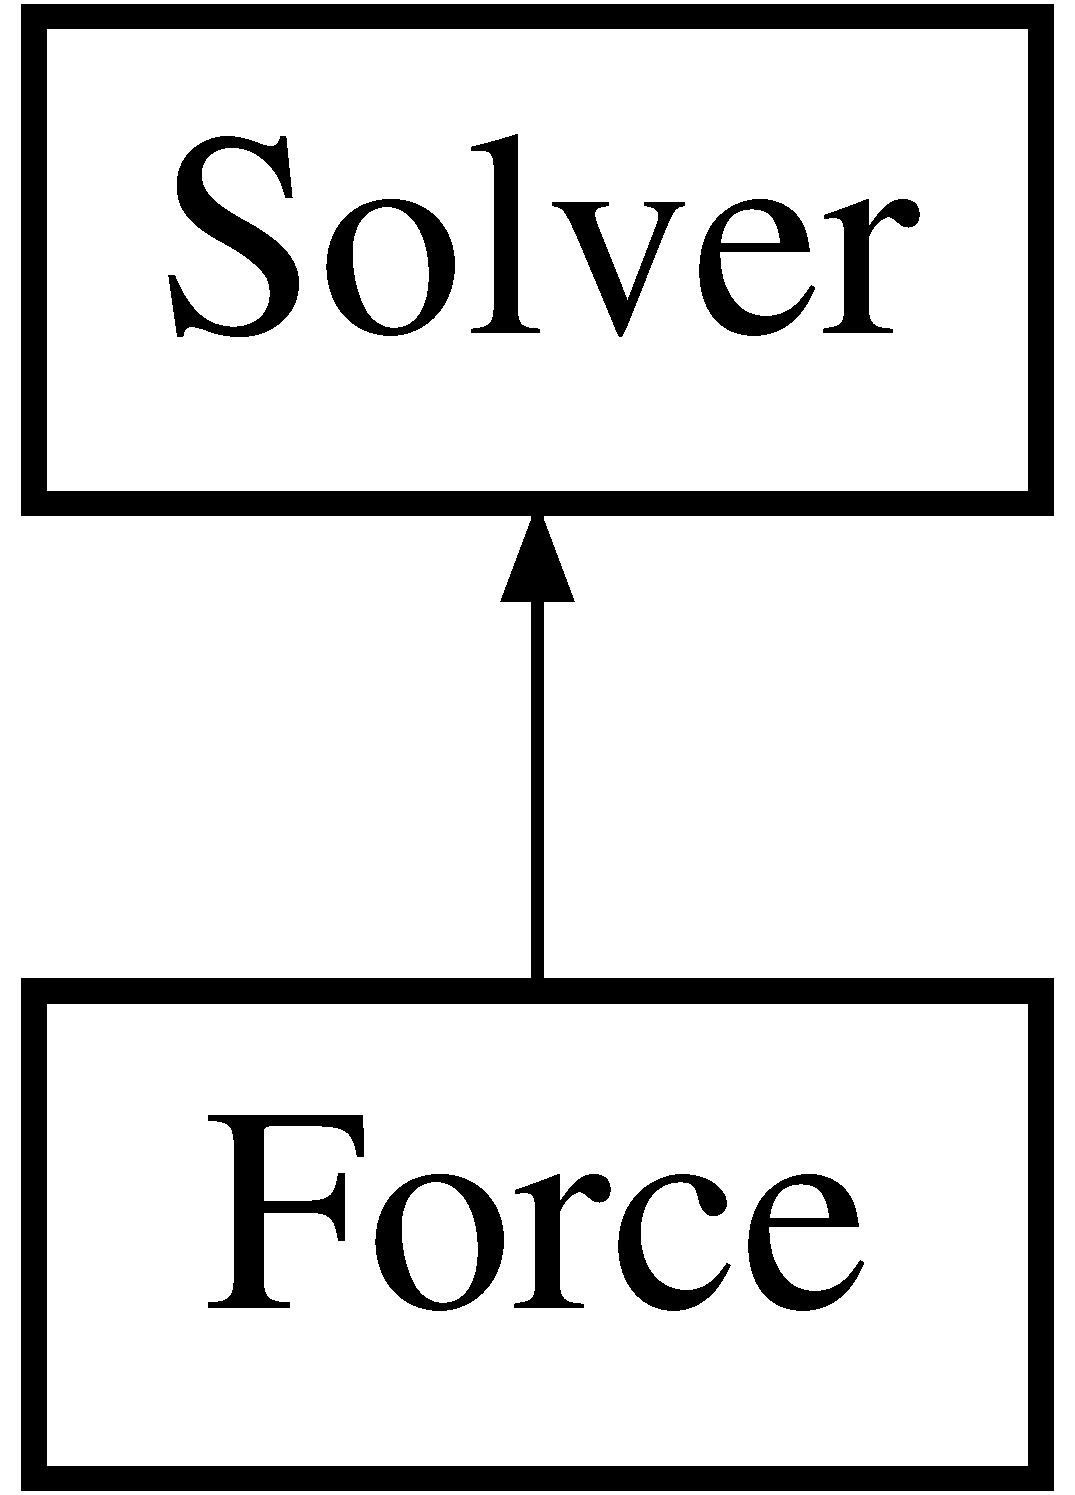
\includegraphics[height=2.000000cm]{classForce}
\end{center}
\end{figure}
\subsection*{Public Member Functions}
\begin{DoxyCompactItemize}
\item 
\hyperlink{classForce_a7649ae54f95bba54f4e15784f92900e6}{Force} (\hyperlink{classConstants}{Constants} $\ast$\hyperlink{classSolver_af8791d3a5042e7be5980ae3247cb60de}{constants}, \hyperlink{classComputation}{Computation} $\ast$\hyperlink{classSolver_a158efd10f04099b8be28561f990b646a}{computation}, \hyperlink{classGrid}{Grid} $\ast$\hyperlink{classSolver_a147ba19192faf8f24dadfc569f3d403f}{grid})
\end{DoxyCompactItemize}
\subsection*{Protected Member Functions}
\begin{DoxyCompactItemize}
\item 
void \hyperlink{classForce_a6c395b2d375796332c6d688760c79dc4}{calc\-\_\-method\-\_\-flux} (double dt, int dir)
\item 
\hypertarget{classForce_ade35a929b504e623e66453f0a3d0cb2a}{void {\bfseries solve\-\_\-1d} (double dt)}\label{classForce_ade35a929b504e623e66453f0a3d0cb2a}

\item 
\hypertarget{classForce_a433b3d8f8ffbb5e3761d7e92397ce2a0}{void {\bfseries solve\-\_\-2d\-\_\-unsplit} (double dt)}\label{classForce_a433b3d8f8ffbb5e3761d7e92397ce2a0}

\item 
\hypertarget{classForce_a3aab917b725dd97e966b41f3dc6c3d8f}{void {\bfseries solve\-\_\-2d\-\_\-split} (double dt)}\label{classForce_a3aab917b725dd97e966b41f3dc6c3d8f}

\end{DoxyCompactItemize}
\subsection*{Protected Attributes}
\begin{DoxyCompactItemize}
\item 
\hypertarget{classForce_a907a325345155efe7b3ba4ec182ede2e}{int {\bfseries neqs}}\label{classForce_a907a325345155efe7b3ba4ec182ede2e}

\item 
\hypertarget{classForce_aee5c074eaaab2b1a4304317628102c78}{double $\ast$ {\bfseries uall}}\label{classForce_aee5c074eaaab2b1a4304317628102c78}

\item 
\hypertarget{classForce_adbb006665c3b6192b8bcd65ad0077e9e}{double $\ast$ {\bfseries fall}}\label{classForce_adbb006665c3b6192b8bcd65ad0077e9e}

\item 
\hypertarget{classForce_a6925da28ddbfbfa5157093d67285ee38}{double $\ast$ {\bfseries gall}}\label{classForce_a6925da28ddbfbfa5157093d67285ee38}

\item 
\hypertarget{classForce_a188408f567873a822d9e63267d613f3c}{double $\ast$ {\bfseries f\-\_\-laxall}}\label{classForce_a188408f567873a822d9e63267d613f3c}

\item 
\hypertarget{classForce_a7180e4de77cf8299a0dd4333057c7d26}{double $\ast$ {\bfseries f\-\_\-rieall}}\label{classForce_a7180e4de77cf8299a0dd4333057c7d26}

\item 
\hypertarget{classForce_a89e725ac253fb6274ce747f93d87c8a0}{double $\ast$ {\bfseries g\-\_\-laxall}}\label{classForce_a89e725ac253fb6274ce747f93d87c8a0}

\item 
\hypertarget{classForce_aaa1af4cc9174fdabf16f8e822c02840a}{double $\ast$ {\bfseries g\-\_\-rieall}}\label{classForce_aaa1af4cc9174fdabf16f8e822c02840a}

\item 
\hypertarget{classForce_a04c220d5edd00045706c95c929086c95}{double $\ast$$\ast$$\ast$ {\bfseries cs}}\label{classForce_a04c220d5edd00045706c95c929086c95}

\item 
\hypertarget{classForce_a94180f5b1cd0087c0fd5c309a1edb747}{double $\ast$$\ast$$\ast$ {\bfseries fd}}\label{classForce_a94180f5b1cd0087c0fd5c309a1edb747}

\item 
\hypertarget{classForce_aee959ad673ab398cc8309322ae42ecd2}{double $\ast$$\ast$$\ast$ {\bfseries gd}}\label{classForce_aee959ad673ab398cc8309322ae42ecd2}

\item 
\hypertarget{classForce_afc58bdb5903d6eafa1740ad762c8b214}{double $\ast$$\ast$$\ast$ {\bfseries f\-\_\-lax}}\label{classForce_afc58bdb5903d6eafa1740ad762c8b214}

\item 
\hypertarget{classForce_a4a43242ebf85eb2d603ea444ec243f8a}{double $\ast$$\ast$$\ast$ {\bfseries f\-\_\-rie}}\label{classForce_a4a43242ebf85eb2d603ea444ec243f8a}

\item 
\hypertarget{classForce_aca3165e40a8789286d288659b7309d28}{double $\ast$$\ast$$\ast$ {\bfseries g\-\_\-lax}}\label{classForce_aca3165e40a8789286d288659b7309d28}

\item 
\hypertarget{classForce_a8f97242d9677a2023e82f906fce096ab}{double $\ast$$\ast$$\ast$ {\bfseries g\-\_\-rie}}\label{classForce_a8f97242d9677a2023e82f906fce096ab}

\item 
\hypertarget{classForce_a192a91d08a845804c681ddfb06b131e3}{double $\ast$$\ast$ {\bfseries f\-\_\-force}}\label{classForce_a192a91d08a845804c681ddfb06b131e3}

\end{DoxyCompactItemize}
\subsection*{Additional Inherited Members}


\subsection{Constructor \& Destructor Documentation}
\hypertarget{classForce_a7649ae54f95bba54f4e15784f92900e6}{\index{Force@{Force}!Force@{Force}}
\index{Force@{Force}!Force@{Force}}
\subsubsection[{Force}]{\setlength{\rightskip}{0pt plus 5cm}Force\-::\-Force (
\begin{DoxyParamCaption}
\item[{{\bf Constants} $\ast$}]{constants, }
\item[{{\bf Computation} $\ast$}]{computation, }
\item[{{\bf Grid} $\ast$}]{grid}
\end{DoxyParamCaption}
)}}\label{classForce_a7649ae54f95bba54f4e15784f92900e6}
Konstruktor der \hyperlink{classFORCE}{F\-O\-R\-C\-E} Methode. Ruft den Konstruktor der geerbten Klasse auf. 
\begin{DoxyParams}{Parameters}
{\em const\-\_\-in} & Dateiname wo \hyperlink{classKonstanten}{Konstanten} gespeichert sind. \\
\hline
{\em formel\-\_\-in} & Dateinamen-\/\-Kern für die Formeln. \\
\hline
{\em save\-\_\-in} & Dateiname wo für das Laden eine Speicherstands die Plots gespeichert sind. \\
\hline
\end{DoxyParams}


\subsection{Member Function Documentation}
\hypertarget{classForce_a6c395b2d375796332c6d688760c79dc4}{\index{Force@{Force}!calc\-\_\-method\-\_\-flux@{calc\-\_\-method\-\_\-flux}}
\index{calc\-\_\-method\-\_\-flux@{calc\-\_\-method\-\_\-flux}!Force@{Force}}
\subsubsection[{calc\-\_\-method\-\_\-flux}]{\setlength{\rightskip}{0pt plus 5cm}void Force\-::calc\-\_\-method\-\_\-flux (
\begin{DoxyParamCaption}
\item[{double}]{dt, }
\item[{int}]{dir}
\end{DoxyParamCaption}
)\hspace{0.3cm}{\ttfamily [protected]}, {\ttfamily [virtual]}}}\label{classForce_a6c395b2d375796332c6d688760c79dc4}
Berechnung des \hyperlink{classFORCE}{F\-O\-R\-C\-E} Flusses. \begin{DoxyReturn}{Returns}
4 Dimensionaler Vektor. Zusammenstellung\-: Gleichung, x-\/\-Position, y-\/\-Position , dimension
\end{DoxyReturn}
Aktualisiert alle zelle mithilfe des berechneten Flusses. Berechnung des \hyperlink{classFORCE}{F\-O\-R\-C\-E} Flusses. \begin{DoxyReturn}{Returns}
4 Dimensionaler Vektor. Zusammenstellung\-: Gleichung, x-\/\-Position, y-\/\-Position , dimension 
\end{DoxyReturn}


Implements \hyperlink{classSolver_ab0c03d26d92272de997fa6984a2a86de}{Solver}.



The documentation for this class was generated from the following files\-:\begin{DoxyCompactItemize}
\item 
force.\-h\item 
force.\-cpp\end{DoxyCompactItemize}

\hypertarget{classGrid}{\section{Grid Class Reference}
\label{classGrid}\index{Grid@{Grid}}
}


{\ttfamily \#include $<$grid.\-h$>$}

\subsection*{Public Member Functions}
\begin{DoxyCompactItemize}
\item 
\hyperlink{classGrid_adf92756bdccf95fc9e3fedac017cc7d0}{Grid} (\hyperlink{classConstants}{Constants} $\ast$\hyperlink{classGrid_a9e529cbb3ec0b42c8b232be05923a030}{constants}, std\-::string save\-\_\-in, int \hyperlink{classGrid_af55897b809ffd9733f6723c8a23d89a5}{choice})
\item 
\hyperlink{classGrid_a01fb58c88ad3ac4a6c2a1eba5742dc7a}{Grid} (int x)
\item 
\hyperlink{classGrid_a338e0b1ffbad1cf5fdf960d7511b4857}{Grid} (int x, int y)
\item 
\hyperlink{classGrid_a3661d0a7f998caaaf8627d7a67072116}{$\sim$\-Grid} ()
\item 
void \hyperlink{classGrid_a1c67c94bc8e4a5dec66934b11129ff63}{init\-\_\-1d\-\_\-rarefaction} ()
\item 
void \hyperlink{classGrid_a491f89e29ba29b1034d4972df9679352}{init\-\_\-1d\-\_\-shockwave} ()
\item 
void \hyperlink{classGrid_a76f8642b671a34b93c195f7266b6e0d4}{init\-\_\-2d\-\_\-rarefaction\-\_\-0} ()
\item 
void \hyperlink{classGrid_a30aa151fda2f732bb542c02a5de26eee}{init\-\_\-2d\-\_\-rarefaction\-\_\-90} ()
\item 
void \hyperlink{classGrid_aff04070089defd8f9100eaff9e6c6fc2}{init\-\_\-2d\-\_\-rarefaction\-\_\-60} ()
\item 
void \hyperlink{classGrid_a3957a41dc0ced492623c46644ca41b4f}{init\-\_\-2d\-\_\-rarefaction\-\_\-45} ()
\item 
void \hyperlink{classGrid_a497011f31b5116f6f691fe2e51c4674d}{init\-\_\-2d\-\_\-shockwave\-\_\-bubble} ()
\item 
void \hyperlink{classGrid_ad2ea723ca3cf2642b3741716fc7c08a7}{init\-\_\-2d\-\_\-load\-\_\-file} (std\-::string save\-\_\-in)
\item 
void \hyperlink{classGrid_a471f6095ce574138fccaff0cad567825}{apply\-\_\-boundary\-\_\-conditions} ()
\end{DoxyCompactItemize}
\subsection*{Public Attributes}
\begin{DoxyCompactItemize}
\item 
int \hyperlink{classGrid_af55897b809ffd9733f6723c8a23d89a5}{choice}
\item 
\hyperlink{classConstants}{Constants} $\ast$ \hyperlink{classGrid_a9e529cbb3ec0b42c8b232be05923a030}{constants}
\item 
double $\ast$$\ast$ \hyperlink{classGrid_aedb9b7d5ce1139730dc73a2f9e0e6edc}{cellsgrid}
\item 
int \hyperlink{classGrid_a6970f8edab2f84c576fc335f6d023f95}{dimension}
\item 
int $\ast$ \hyperlink{classGrid_a7b4eea4e828ebda3ebdfe78b2f9a14d2}{grid\-\_\-size}
\item 
int $\ast$ \hyperlink{classGrid_adbf3823ea45f6e5ae9210d44fbc7e79a}{grid\-\_\-size\-\_\-total}
\item 
int $\ast$ \hyperlink{classGrid_a68bd279fd3b1cee412e436b1f3848225}{boundary\-\_\-conditions}
\item 
int \hyperlink{classGrid_a599c5aadae9322d115d974cb395a83bf}{orderofgrid}
\item 
int \hyperlink{classGrid_a2f725f73b6290e8c8527a6566ef07895}{cellsgrid\-\_\-size}
\end{DoxyCompactItemize}


\subsection{Detailed Description}
Diese Klasse bietet ein Raster aus Zellen. Zellen werden in einem 1-\/\-Dimensionalen Array abgespeichert, welches dann auch noch falls nötig 2-\/\-Dimensional oder 3-\/\-Dimensional interpretiert wird. 

\subsection{Constructor \& Destructor Documentation}
\hypertarget{classGrid_adf92756bdccf95fc9e3fedac017cc7d0}{\index{Grid@{Grid}!Grid@{Grid}}
\index{Grid@{Grid}!Grid@{Grid}}
\subsubsection[{Grid}]{\setlength{\rightskip}{0pt plus 5cm}Grid\-::\-Grid (
\begin{DoxyParamCaption}
\item[{{\bf Constants} $\ast$}]{constants, }
\item[{std\-::string}]{save\-\_\-in, }
\item[{int}]{choice}
\end{DoxyParamCaption}
)}}\label{classGrid_adf92756bdccf95fc9e3fedac017cc7d0}
Konstruktor des Rasters. 
\begin{DoxyParams}{Parameters}
{\em constants} & Pointer auf das Objekt, welches die \hyperlink{classKonstanten}{Konstanten} enthält. \\
\hline
{\em save\-\_\-in} & Pfad zur Datei mit dem Speicherstand. \\
\hline
{\em choice} & Gibt die zu verwendende Initialisierungsmethode an \\
\hline
\end{DoxyParams}
\hypertarget{classGrid_a01fb58c88ad3ac4a6c2a1eba5742dc7a}{\index{Grid@{Grid}!Grid@{Grid}}
\index{Grid@{Grid}!Grid@{Grid}}
\subsubsection[{Grid}]{\setlength{\rightskip}{0pt plus 5cm}Grid\-::\-Grid (
\begin{DoxyParamCaption}
\item[{int}]{x}
\end{DoxyParamCaption}
)}}\label{classGrid_a01fb58c88ad3ac4a6c2a1eba5742dc7a}
Konstruktor für ein leeres eindimensionales Raster. \hypertarget{classGrid_a338e0b1ffbad1cf5fdf960d7511b4857}{\index{Grid@{Grid}!Grid@{Grid}}
\index{Grid@{Grid}!Grid@{Grid}}
\subsubsection[{Grid}]{\setlength{\rightskip}{0pt plus 5cm}Grid\-::\-Grid (
\begin{DoxyParamCaption}
\item[{int}]{x, }
\item[{int}]{y}
\end{DoxyParamCaption}
)}}\label{classGrid_a338e0b1ffbad1cf5fdf960d7511b4857}
Konstruktor für ein leeres zweidimensionales Raster. \hypertarget{classGrid_a3661d0a7f998caaaf8627d7a67072116}{\index{Grid@{Grid}!$\sim$\-Grid@{$\sim$\-Grid}}
\index{$\sim$\-Grid@{$\sim$\-Grid}!Grid@{Grid}}
\subsubsection[{$\sim$\-Grid}]{\setlength{\rightskip}{0pt plus 5cm}Grid\-::$\sim$\-Grid (
\begin{DoxyParamCaption}
{}
\end{DoxyParamCaption}
)}}\label{classGrid_a3661d0a7f998caaaf8627d7a67072116}
Destruktor des Rasters. Gibt alokierten Speicher wieder frei.

Destruktor 

\subsection{Member Function Documentation}
\hypertarget{classGrid_a471f6095ce574138fccaff0cad567825}{\index{Grid@{Grid}!apply\-\_\-boundary\-\_\-conditions@{apply\-\_\-boundary\-\_\-conditions}}
\index{apply\-\_\-boundary\-\_\-conditions@{apply\-\_\-boundary\-\_\-conditions}!Grid@{Grid}}
\subsubsection[{apply\-\_\-boundary\-\_\-conditions}]{\setlength{\rightskip}{0pt plus 5cm}void Grid\-::apply\-\_\-boundary\-\_\-conditions (
\begin{DoxyParamCaption}
{}
\end{DoxyParamCaption}
)}}\label{classGrid_a471f6095ce574138fccaff0cad567825}
Wendet Randbedingungen an. 
\begin{DoxyParams}{Parameters}
{\em konstanten} & \hyperlink{classKonstanten}{Konstanten} wo festgelegt ist welche Randbedingungen angewendet werden.\\
\hline
\end{DoxyParams}
Anwenden der Randbedingungen \hypertarget{classGrid_a1c67c94bc8e4a5dec66934b11129ff63}{\index{Grid@{Grid}!init\-\_\-1d\-\_\-rarefaction@{init\-\_\-1d\-\_\-rarefaction}}
\index{init\-\_\-1d\-\_\-rarefaction@{init\-\_\-1d\-\_\-rarefaction}!Grid@{Grid}}
\subsubsection[{init\-\_\-1d\-\_\-rarefaction}]{\setlength{\rightskip}{0pt plus 5cm}void Grid\-::init\-\_\-1d\-\_\-rarefaction (
\begin{DoxyParamCaption}
{}
\end{DoxyParamCaption}
)}}\label{classGrid_a1c67c94bc8e4a5dec66934b11129ff63}
Initialisierungsmethode für eine Verdünnungswelle auf einem 1\-D-\/\-Raster \hypertarget{classGrid_a491f89e29ba29b1034d4972df9679352}{\index{Grid@{Grid}!init\-\_\-1d\-\_\-shockwave@{init\-\_\-1d\-\_\-shockwave}}
\index{init\-\_\-1d\-\_\-shockwave@{init\-\_\-1d\-\_\-shockwave}!Grid@{Grid}}
\subsubsection[{init\-\_\-1d\-\_\-shockwave}]{\setlength{\rightskip}{0pt plus 5cm}void Grid\-::init\-\_\-1d\-\_\-shockwave (
\begin{DoxyParamCaption}
{}
\end{DoxyParamCaption}
)}}\label{classGrid_a491f89e29ba29b1034d4972df9679352}
Initialisierungsmethode für eine Schockwelle auf einem 1\-D-\/\-Raster \hypertarget{classGrid_ad2ea723ca3cf2642b3741716fc7c08a7}{\index{Grid@{Grid}!init\-\_\-2d\-\_\-load\-\_\-file@{init\-\_\-2d\-\_\-load\-\_\-file}}
\index{init\-\_\-2d\-\_\-load\-\_\-file@{init\-\_\-2d\-\_\-load\-\_\-file}!Grid@{Grid}}
\subsubsection[{init\-\_\-2d\-\_\-load\-\_\-file}]{\setlength{\rightskip}{0pt plus 5cm}void Grid\-::init\-\_\-2d\-\_\-load\-\_\-file (
\begin{DoxyParamCaption}
\item[{std\-::string}]{save\-\_\-in}
\end{DoxyParamCaption}
)}}\label{classGrid_ad2ea723ca3cf2642b3741716fc7c08a7}
Initialisierungsmethode mit einem Speicherstand auf einem 2\-D-\/\-Raster \hypertarget{classGrid_a76f8642b671a34b93c195f7266b6e0d4}{\index{Grid@{Grid}!init\-\_\-2d\-\_\-rarefaction\-\_\-0@{init\-\_\-2d\-\_\-rarefaction\-\_\-0}}
\index{init\-\_\-2d\-\_\-rarefaction\-\_\-0@{init\-\_\-2d\-\_\-rarefaction\-\_\-0}!Grid@{Grid}}
\subsubsection[{init\-\_\-2d\-\_\-rarefaction\-\_\-0}]{\setlength{\rightskip}{0pt plus 5cm}void Grid\-::init\-\_\-2d\-\_\-rarefaction\-\_\-0 (
\begin{DoxyParamCaption}
{}
\end{DoxyParamCaption}
)}}\label{classGrid_a76f8642b671a34b93c195f7266b6e0d4}
Initialisierungsmethode für eine Verdünnungswelle in X-\/\-Richtung auf einem 2\-D-\/\-Raster \hypertarget{classGrid_a3957a41dc0ced492623c46644ca41b4f}{\index{Grid@{Grid}!init\-\_\-2d\-\_\-rarefaction\-\_\-45@{init\-\_\-2d\-\_\-rarefaction\-\_\-45}}
\index{init\-\_\-2d\-\_\-rarefaction\-\_\-45@{init\-\_\-2d\-\_\-rarefaction\-\_\-45}!Grid@{Grid}}
\subsubsection[{init\-\_\-2d\-\_\-rarefaction\-\_\-45}]{\setlength{\rightskip}{0pt plus 5cm}void Grid\-::init\-\_\-2d\-\_\-rarefaction\-\_\-45 (
\begin{DoxyParamCaption}
{}
\end{DoxyParamCaption}
)}}\label{classGrid_a3957a41dc0ced492623c46644ca41b4f}
Initialisierungsmethode für eine Verdünnungswelle in einem 45 Grad Winkel auf einem 2\-D-\/\-Raster \hypertarget{classGrid_aff04070089defd8f9100eaff9e6c6fc2}{\index{Grid@{Grid}!init\-\_\-2d\-\_\-rarefaction\-\_\-60@{init\-\_\-2d\-\_\-rarefaction\-\_\-60}}
\index{init\-\_\-2d\-\_\-rarefaction\-\_\-60@{init\-\_\-2d\-\_\-rarefaction\-\_\-60}!Grid@{Grid}}
\subsubsection[{init\-\_\-2d\-\_\-rarefaction\-\_\-60}]{\setlength{\rightskip}{0pt plus 5cm}void Grid\-::init\-\_\-2d\-\_\-rarefaction\-\_\-60 (
\begin{DoxyParamCaption}
{}
\end{DoxyParamCaption}
)}}\label{classGrid_aff04070089defd8f9100eaff9e6c6fc2}
Initialisierungsmethode für eine Verdünnungswelle in einem 60 Grad Winkel auf einem 2\-D-\/\-Raster \hypertarget{classGrid_a30aa151fda2f732bb542c02a5de26eee}{\index{Grid@{Grid}!init\-\_\-2d\-\_\-rarefaction\-\_\-90@{init\-\_\-2d\-\_\-rarefaction\-\_\-90}}
\index{init\-\_\-2d\-\_\-rarefaction\-\_\-90@{init\-\_\-2d\-\_\-rarefaction\-\_\-90}!Grid@{Grid}}
\subsubsection[{init\-\_\-2d\-\_\-rarefaction\-\_\-90}]{\setlength{\rightskip}{0pt plus 5cm}void Grid\-::init\-\_\-2d\-\_\-rarefaction\-\_\-90 (
\begin{DoxyParamCaption}
{}
\end{DoxyParamCaption}
)}}\label{classGrid_a30aa151fda2f732bb542c02a5de26eee}
Initialisierungsmethode für eine Verdünnungswelle in Y-\/\-Richtung auf einem 2\-D-\/\-Raster \hypertarget{classGrid_a497011f31b5116f6f691fe2e51c4674d}{\index{Grid@{Grid}!init\-\_\-2d\-\_\-shockwave\-\_\-bubble@{init\-\_\-2d\-\_\-shockwave\-\_\-bubble}}
\index{init\-\_\-2d\-\_\-shockwave\-\_\-bubble@{init\-\_\-2d\-\_\-shockwave\-\_\-bubble}!Grid@{Grid}}
\subsubsection[{init\-\_\-2d\-\_\-shockwave\-\_\-bubble}]{\setlength{\rightskip}{0pt plus 5cm}void Grid\-::init\-\_\-2d\-\_\-shockwave\-\_\-bubble (
\begin{DoxyParamCaption}
{}
\end{DoxyParamCaption}
)}}\label{classGrid_a497011f31b5116f6f691fe2e51c4674d}
Initialisierungsmethode für eine Schockwelle-\/auf-\/\-Blase-\/\-Simulation auf einem 2\-D-\/\-Raster 

\subsection{Member Data Documentation}
\hypertarget{classGrid_a68bd279fd3b1cee412e436b1f3848225}{\index{Grid@{Grid}!boundary\-\_\-conditions@{boundary\-\_\-conditions}}
\index{boundary\-\_\-conditions@{boundary\-\_\-conditions}!Grid@{Grid}}
\subsubsection[{boundary\-\_\-conditions}]{\setlength{\rightskip}{0pt plus 5cm}int$\ast$ Grid\-::boundary\-\_\-conditions}}\label{classGrid_a68bd279fd3b1cee412e436b1f3848225}
Dynamisch angelegtes Array je nach Dimension, dass die Art der Boundary Condition speichert \mbox{[}0\mbox{]} kleinster X-\/\-Wert, \mbox{[}1\mbox{]} größter X-\/\-Wert, \mbox{[}2\mbox{]} kleinster Y-\/\-Wert, ... \hypertarget{classGrid_aedb9b7d5ce1139730dc73a2f9e0e6edc}{\index{Grid@{Grid}!cellsgrid@{cellsgrid}}
\index{cellsgrid@{cellsgrid}!Grid@{Grid}}
\subsubsection[{cellsgrid}]{\setlength{\rightskip}{0pt plus 5cm}double$\ast$$\ast$ Grid\-::cellsgrid}}\label{classGrid_aedb9b7d5ce1139730dc73a2f9e0e6edc}
Zellen werden in einem 2-\/dimensionalen Array abgespeichert. Die erste Dimension entspricht der Position und wird dann je nach Dimension des Rasters interpretiert. Die zweite Dimension entspricht den Zellwerten in der Reihenfolge\-: d, p, ux, uxr, uy, ... \hypertarget{classGrid_a2f725f73b6290e8c8527a6566ef07895}{\index{Grid@{Grid}!cellsgrid\-\_\-size@{cellsgrid\-\_\-size}}
\index{cellsgrid\-\_\-size@{cellsgrid\-\_\-size}!Grid@{Grid}}
\subsubsection[{cellsgrid\-\_\-size}]{\setlength{\rightskip}{0pt plus 5cm}int Grid\-::cellsgrid\-\_\-size}}\label{classGrid_a2f725f73b6290e8c8527a6566ef07895}
Anzahl der Zellen \hypertarget{classGrid_af55897b809ffd9733f6723c8a23d89a5}{\index{Grid@{Grid}!choice@{choice}}
\index{choice@{choice}!Grid@{Grid}}
\subsubsection[{choice}]{\setlength{\rightskip}{0pt plus 5cm}int Grid\-::choice}}\label{classGrid_af55897b809ffd9733f6723c8a23d89a5}
Wahl der Initialisierungsmethode des Rasters. \hypertarget{classGrid_a9e529cbb3ec0b42c8b232be05923a030}{\index{Grid@{Grid}!constants@{constants}}
\index{constants@{constants}!Grid@{Grid}}
\subsubsection[{constants}]{\setlength{\rightskip}{0pt plus 5cm}{\bf Constants}$\ast$ Grid\-::constants}}\label{classGrid_a9e529cbb3ec0b42c8b232be05923a030}
Pointer auf ein Objekt mit allen \hyperlink{classKonstanten}{Konstanten}, welche für die Berechnungen benötigt werden \begin{DoxySeeAlso}{See Also}
\hyperlink{classConstants}{Constants} 
\end{DoxySeeAlso}
\hypertarget{classGrid_a6970f8edab2f84c576fc335f6d023f95}{\index{Grid@{Grid}!dimension@{dimension}}
\index{dimension@{dimension}!Grid@{Grid}}
\subsubsection[{dimension}]{\setlength{\rightskip}{0pt plus 5cm}int Grid\-::dimension}}\label{classGrid_a6970f8edab2f84c576fc335f6d023f95}
Dimension des Rasters (Maximal 3). \hypertarget{classGrid_a7b4eea4e828ebda3ebdfe78b2f9a14d2}{\index{Grid@{Grid}!grid\-\_\-size@{grid\-\_\-size}}
\index{grid\-\_\-size@{grid\-\_\-size}!Grid@{Grid}}
\subsubsection[{grid\-\_\-size}]{\setlength{\rightskip}{0pt plus 5cm}int$\ast$ Grid\-::grid\-\_\-size}}\label{classGrid_a7b4eea4e828ebda3ebdfe78b2f9a14d2}
Anzahl der Zellen ohne Grenze \mbox{[}0\mbox{]} height / \mbox{[}1\mbox{]} width / \mbox{[}2\mbox{]} depth \hypertarget{classGrid_adbf3823ea45f6e5ae9210d44fbc7e79a}{\index{Grid@{Grid}!grid\-\_\-size\-\_\-total@{grid\-\_\-size\-\_\-total}}
\index{grid\-\_\-size\-\_\-total@{grid\-\_\-size\-\_\-total}!Grid@{Grid}}
\subsubsection[{grid\-\_\-size\-\_\-total}]{\setlength{\rightskip}{0pt plus 5cm}int$\ast$ Grid\-::grid\-\_\-size\-\_\-total}}\label{classGrid_adbf3823ea45f6e5ae9210d44fbc7e79a}
Anzahl der Zellenränder (+ 1) mit Grenze (ordnung $\ast$ 2) \mbox{[}0\mbox{]} Breite \mbox{[}1\mbox{]} Weite \mbox{[}2\mbox{]} Tiefe \hypertarget{classGrid_a599c5aadae9322d115d974cb395a83bf}{\index{Grid@{Grid}!orderofgrid@{orderofgrid}}
\index{orderofgrid@{orderofgrid}!Grid@{Grid}}
\subsubsection[{orderofgrid}]{\setlength{\rightskip}{0pt plus 5cm}int Grid\-::orderofgrid}}\label{classGrid_a599c5aadae9322d115d974cb395a83bf}
Ordnung des Rasters Gibt an wie viele Nachbarwerte (pro Seite) miteinbezogen werden sollen 

The documentation for this class was generated from the following files\-:\begin{DoxyCompactItemize}
\item 
grid.\-h\item 
grid.\-cpp\end{DoxyCompactItemize}

\hypertarget{classKonstanten}{\section{Konstanten Class Reference}
\label{classKonstanten}\index{Konstanten@{Konstanten}}
}


{\ttfamily \#include $<$Konstanten.\-h$>$}

\subsection*{Public Member Functions}
\begin{DoxyCompactItemize}
\item 
\hyperlink{classKonstanten_a4a5a2fac8680b4cf055029be43f4c18c}{Konstanten} (std\-::string input\-\_\-const)
\end{DoxyCompactItemize}
\subsection*{Public Attributes}
\begin{DoxyCompactItemize}
\item 
std\-::vector$<$ std\-::string $>$ \hyperlink{classKonstanten_abd044489471f59656078d51706353bf5}{const\-\_\-name}
\item 
std\-::vector$<$ double $>$ \hyperlink{classKonstanten_a12dc216c8d055e95ed17d819a5949832}{const\-\_\-value}
\item 
\hypertarget{classKonstanten_a79a04aec0180007251b811999e5107b8}{int {\bfseries calceigv}}\label{classKonstanten_a79a04aec0180007251b811999e5107b8}

\item 
\hypertarget{classKonstanten_a2cfd196ff2e81d46929c3efdd00ec62c}{int {\bfseries variante}}\label{classKonstanten_a2cfd196ff2e81d46929c3efdd00ec62c}

\item 
\hypertarget{classKonstanten_a987274e0e5793520b7a445ed9873c3bf}{double {\bfseries teiler}}\label{classKonstanten_a987274e0e5793520b7a445ed9873c3bf}

\item 
\hypertarget{classKonstanten_ae3edf7d78df231706cf8e76244391cab}{int {\bfseries teilerend}}\label{classKonstanten_ae3edf7d78df231706cf8e76244391cab}

\item 
\hypertarget{classKonstanten_a84dfdf3a59e6c5affa98be399569b01a}{double {\bfseries timeou}}\label{classKonstanten_a84dfdf3a59e6c5affa98be399569b01a}

\item 
\hypertarget{classKonstanten_a028517c1cbc7e062a31fb7d204f64a96}{double {\bfseries cfl}}\label{classKonstanten_a028517c1cbc7e062a31fb7d204f64a96}

\item 
\hypertarget{classKonstanten_af02b3d81b23fb756a7821550f17f5817}{int {\bfseries maxnt}}\label{classKonstanten_af02b3d81b23fb756a7821550f17f5817}

\item 
\hypertarget{classKonstanten_ad24e5c861894ff6df3368fbe28ecee56}{int {\bfseries dimension}}\label{classKonstanten_ad24e5c861894ff6df3368fbe28ecee56}

\item 
\hypertarget{classKonstanten_a2d407c35f20f0bf27c2152ed67cb0851}{int {\bfseries ordnung}}\label{classKonstanten_a2d407c35f20f0bf27c2152ed67cb0851}

\item 
\hypertarget{classKonstanten_a3f97bdddf7c7bad19afb456167496471}{double {\bfseries radius}}\label{classKonstanten_a3f97bdddf7c7bad19afb456167496471}

\item 
\hypertarget{classKonstanten_af28f753eda4f33bee6be6844519641ed}{int {\bfseries C\-E\-L\-L\-S\-X}}\label{classKonstanten_af28f753eda4f33bee6be6844519641ed}

\item 
\hypertarget{classKonstanten_aa68cbb100282389bd7fc9efdc5cf04da}{int {\bfseries C\-E\-L\-L\-S\-Y}}\label{classKonstanten_aa68cbb100282389bd7fc9efdc5cf04da}

\item 
\hypertarget{classKonstanten_a8e03c316cd153326b83120e7f69ac9cc}{double {\bfseries g}}\label{classKonstanten_a8e03c316cd153326b83120e7f69ac9cc}

\item 
\hypertarget{classKonstanten_a7a48e3cf7787f8a77f6fa0d073967229}{double {\bfseries mol}}\label{classKonstanten_a7a48e3cf7787f8a77f6fa0d073967229}

\item 
\hypertarget{classKonstanten_ad0f8a36eab29909dbe37d1baf9db3542}{double {\bfseries mor}}\label{classKonstanten_ad0f8a36eab29909dbe37d1baf9db3542}

\item 
\hypertarget{classKonstanten_af1912a9942b66bc8e2965840f0dcef08}{double {\bfseries mul}}\label{classKonstanten_af1912a9942b66bc8e2965840f0dcef08}

\item 
\hypertarget{classKonstanten_a062ce50d35bd692ab4b492cf40225ff3}{double {\bfseries mur}}\label{classKonstanten_a062ce50d35bd692ab4b492cf40225ff3}

\item 
\hypertarget{classKonstanten_a7a85280fdf83d10bf3a14f3f772bef2a}{int {\bfseries upbc}}\label{classKonstanten_a7a85280fdf83d10bf3a14f3f772bef2a}

\item 
\hypertarget{classKonstanten_a55f2f34f199cf5c377280272350695c4}{int {\bfseries downbc}}\label{classKonstanten_a55f2f34f199cf5c377280272350695c4}

\item 
\hypertarget{classKonstanten_a1906cb7c990779e92707cc752358e7ca}{int {\bfseries leftbc}}\label{classKonstanten_a1906cb7c990779e92707cc752358e7ca}

\item 
\hypertarget{classKonstanten_aedc6f7a6f365ad1c42b0bb58c14d0d5f}{int {\bfseries rightbc}}\label{classKonstanten_aedc6f7a6f365ad1c42b0bb58c14d0d5f}

\item 
\hypertarget{classKonstanten_a8a8ba974eadebfd1baa2d7246d1eadf8}{double {\bfseries cref}}\label{classKonstanten_a8a8ba974eadebfd1baa2d7246d1eadf8}

\item 
\hypertarget{classKonstanten_a45f2dc4cdb262f34f256f0418b2d9b20}{double {\bfseries done}}\label{classKonstanten_a45f2dc4cdb262f34f256f0418b2d9b20}

\item 
\hypertarget{classKonstanten_a4fd1dc55cc0b72a05426aae1cf0b3902}{double {\bfseries ccl}}\label{classKonstanten_a4fd1dc55cc0b72a05426aae1cf0b3902}

\item 
\hypertarget{classKonstanten_aba36196bc1a291ad9176f73c0b607677}{double {\bfseries rhol}}\label{classKonstanten_aba36196bc1a291ad9176f73c0b607677}

\item 
\hypertarget{classKonstanten_aec1cce17aadacf240ace975f68727f21}{double {\bfseries vl}}\label{classKonstanten_aec1cce17aadacf240ace975f68727f21}

\item 
\hypertarget{classKonstanten_a44b6880e75797d69346c5c8212124952}{double {\bfseries vrl}}\label{classKonstanten_a44b6880e75797d69346c5c8212124952}

\item 
\hypertarget{classKonstanten_a8a9d76a1177266158c2fa3900484d244}{double {\bfseries vyl}}\label{classKonstanten_a8a9d76a1177266158c2fa3900484d244}

\item 
\hypertarget{classKonstanten_ac4bd60cb7712a4230c70a8d1d481c8ec}{double {\bfseries vyrl}}\label{classKonstanten_ac4bd60cb7712a4230c70a8d1d481c8ec}

\item 
\hypertarget{classKonstanten_ae1a2831635cbd559716dca269849823b}{double {\bfseries rhor}}\label{classKonstanten_ae1a2831635cbd559716dca269849823b}

\item 
\hypertarget{classKonstanten_a45cb5090ba21586b7db67424f2ac9e97}{double {\bfseries vr}}\label{classKonstanten_a45cb5090ba21586b7db67424f2ac9e97}

\item 
\hypertarget{classKonstanten_afc3cd7105f50e81e25277cdd902b2410}{double {\bfseries vrr}}\label{classKonstanten_afc3cd7105f50e81e25277cdd902b2410}

\item 
\hypertarget{classKonstanten_a326d4d4c71f750ef4a0173669634b770}{double {\bfseries vyr}}\label{classKonstanten_a326d4d4c71f750ef4a0173669634b770}

\item 
\hypertarget{classKonstanten_a83f4e7a4cfc3087cb683d556d178951a}{double {\bfseries vyrr}}\label{classKonstanten_a83f4e7a4cfc3087cb683d556d178951a}

\end{DoxyCompactItemize}


\subsection{Detailed Description}
Die Klasse \hyperlink{classKonstanten}{Konstanten} dient hauptsächlich dazu sämtliche für Berechnungen benötigte \hyperlink{classKonstanten}{Konstanten} zusammenzufassen und leicht für Rechnungen verfügbar zu machen. 

\subsection{Constructor \& Destructor Documentation}
\hypertarget{classKonstanten_a4a5a2fac8680b4cf055029be43f4c18c}{\index{Konstanten@{Konstanten}!Konstanten@{Konstanten}}
\index{Konstanten@{Konstanten}!Konstanten@{Konstanten}}
\subsubsection[{Konstanten}]{\setlength{\rightskip}{0pt plus 5cm}Konstanten\-::\-Konstanten (
\begin{DoxyParamCaption}
\item[{std\-::string}]{input\-\_\-const}
\end{DoxyParamCaption}
)}}\label{classKonstanten_a4a5a2fac8680b4cf055029be43f4c18c}
Konstruktor. Setzt die \hyperlink{classKonstanten}{Konstanten}. 
\begin{DoxyParams}{Parameters}
{\em input\-\_\-const} & String des Pfades zu den festen \hyperlink{classKonstanten}{Konstanten}. \\
\hline
{\em input\-\_\-calc} & String des Pfades zu den einmalig zu berechnenden \hyperlink{classKonstanten}{Konstanten}.\\
\hline
\end{DoxyParams}
Konstruktor. 
\begin{DoxyParams}{Parameters}
{\em input\-\_\-const} & String des Pfades zu den festen \hyperlink{classKonstanten}{Konstanten}. \\
\hline
{\em input\-\_\-calc} & String des Pfades zu den einmalig zu berechnenden \hyperlink{classKonstanten}{Konstanten}. \\
\hline
\end{DoxyParams}


\subsection{Member Data Documentation}
\hypertarget{classKonstanten_abd044489471f59656078d51706353bf5}{\index{Konstanten@{Konstanten}!const\-\_\-name@{const\-\_\-name}}
\index{const\-\_\-name@{const\-\_\-name}!Konstanten@{Konstanten}}
\subsubsection[{const\-\_\-name}]{\setlength{\rightskip}{0pt plus 5cm}std\-::vector$<$std\-::string$>$ Konstanten\-::const\-\_\-name}}\label{classKonstanten_abd044489471f59656078d51706353bf5}
Beizeichnungen der \hyperlink{classKonstanten}{Konstanten} in einem Vektor. \hypertarget{classKonstanten_a12dc216c8d055e95ed17d819a5949832}{\index{Konstanten@{Konstanten}!const\-\_\-value@{const\-\_\-value}}
\index{const\-\_\-value@{const\-\_\-value}!Konstanten@{Konstanten}}
\subsubsection[{const\-\_\-value}]{\setlength{\rightskip}{0pt plus 5cm}std\-::vector$<$double$>$ Konstanten\-::const\-\_\-value}}\label{classKonstanten_a12dc216c8d055e95ed17d819a5949832}
Vektor von Werten der \hyperlink{classKonstanten}{Konstanten}. 

The documentation for this class was generated from the following files\-:\begin{DoxyCompactItemize}
\item 
Konstanten.\-h\item 
Konstanten.\-cpp\end{DoxyCompactItemize}

\hypertarget{classLax__Friedrich}{\section{Lax\-\_\-\-Friedrich Class Reference}
\label{classLax__Friedrich}\index{Lax\-\_\-\-Friedrich@{Lax\-\_\-\-Friedrich}}
}


{\ttfamily \#include $<$lax\-\_\-friedrich.\-h$>$}

Inheritance diagram for Lax\-\_\-\-Friedrich\-:\begin{figure}[H]
\begin{center}
\leavevmode
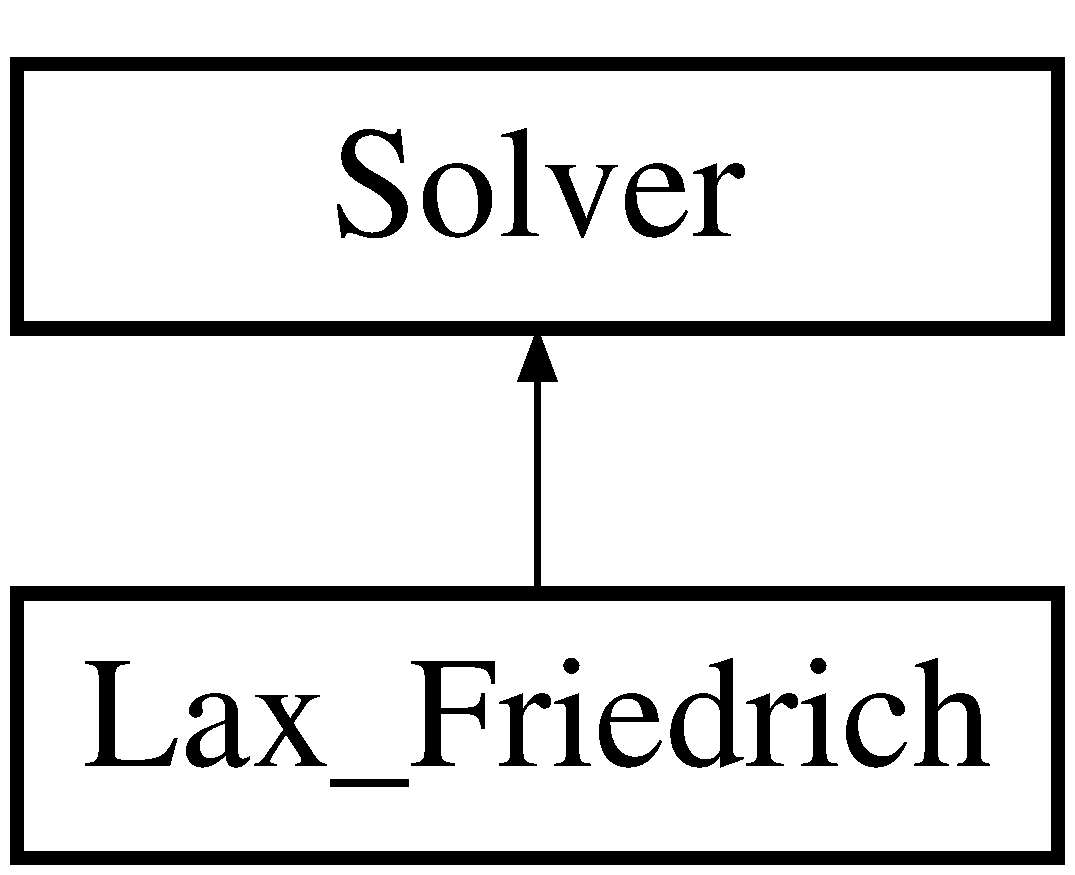
\includegraphics[height=2.000000cm]{classLax__Friedrich}
\end{center}
\end{figure}
\subsection*{Public Member Functions}
\begin{DoxyCompactItemize}
\item 
\hyperlink{classLax__Friedrich_ae81b6a1af98230c75ed8f11b99f95532}{Lax\-\_\-\-Friedrich} (\hyperlink{classConstants}{Constants} $\ast$\hyperlink{classSolver_af8791d3a5042e7be5980ae3247cb60de}{constants}, \hyperlink{classComputation}{Computation} $\ast$\hyperlink{classSolver_a158efd10f04099b8be28561f990b646a}{computation}, \hyperlink{classGrid}{Grid} $\ast$\hyperlink{classSolver_a147ba19192faf8f24dadfc569f3d403f}{grid})
\item 
virtual \hyperlink{classLax__Friedrich_ad069bf434093eba9f5fa1c6d02d93dfd}{$\sim$\-Lax\-\_\-\-Friedrich} ()
\item 
void \hyperlink{classLax__Friedrich_aff4e2d9fd2a38de402e96ce4f0e1c1bc}{solve\-\_\-1d} (double dt)
\item 
void \hyperlink{classLax__Friedrich_ae7aff2026dbcc2a731119a5ff541b4ab}{solve\-\_\-2d\-\_\-unsplit} (double dt)
\item 
void \hyperlink{classLax__Friedrich_a0086e60fef8bbb1d8ba1cd5b228a90f6}{solve\-\_\-2d\-\_\-split} (double dt)
\end{DoxyCompactItemize}
\subsection*{Protected Member Functions}
\begin{DoxyCompactItemize}
\item 
void \hyperlink{classLax__Friedrich_a77ace0aa368e5b04263b23a69d2b3fe7}{calc\-\_\-method\-\_\-flux} (double dt, int dir)
\end{DoxyCompactItemize}
\subsection*{Protected Attributes}
\begin{DoxyCompactItemize}
\item 
int \hyperlink{classLax__Friedrich_a54f821dda8e829ce85adc3afc77dce49}{neqs}
\item 
double $\ast$ \hyperlink{classLax__Friedrich_a46da19f1f8569252fde5ab59c357859c}{uall}
\item 
double $\ast$ \hyperlink{classLax__Friedrich_ad04ba32ac42deeae836e2acc594f7b52}{fall}
\item 
double $\ast$ \hyperlink{classLax__Friedrich_a46a918bceab80d7a6f2042a2e96cf4bd}{gall}
\item 
double $\ast$$\ast$$\ast$ \hyperlink{classLax__Friedrich_ae3409552d0a7e6e2168d7292183f2509}{cs}
\item 
double $\ast$$\ast$$\ast$ \hyperlink{classLax__Friedrich_a2e593b52e256ab0be6cf06eed59566e7}{f}
\item 
double $\ast$$\ast$$\ast$ \hyperlink{classLax__Friedrich_a78574df783b04827507ad183522ee021}{g}
\item 
double $\ast$$\ast$ \hyperlink{classLax__Friedrich_a007ddad79c40ef536d303cbe136dfdb6}{f\-\_\-lax}
\end{DoxyCompactItemize}
\subsection*{Additional Inherited Members}


\subsection{Detailed Description}
Klasse der Lax-\/\-Friedrichs Methode. Die Berechnung des Lax-\/\-Friedrich Flusses wird hier spezialisiert, erbt von der Klasse \hyperlink{classSolver}{Solver} 

\subsection{Constructor \& Destructor Documentation}
\hypertarget{classLax__Friedrich_ae81b6a1af98230c75ed8f11b99f95532}{\index{Lax\-\_\-\-Friedrich@{Lax\-\_\-\-Friedrich}!Lax\-\_\-\-Friedrich@{Lax\-\_\-\-Friedrich}}
\index{Lax\-\_\-\-Friedrich@{Lax\-\_\-\-Friedrich}!Lax_Friedrich@{Lax\-\_\-\-Friedrich}}
\subsubsection[{Lax\-\_\-\-Friedrich}]{\setlength{\rightskip}{0pt plus 5cm}Lax\-\_\-\-Friedrich\-::\-Lax\-\_\-\-Friedrich (
\begin{DoxyParamCaption}
\item[{{\bf Constants} $\ast$}]{constants, }
\item[{{\bf Computation} $\ast$}]{computation, }
\item[{{\bf Grid} $\ast$}]{grid}
\end{DoxyParamCaption}
)}}\label{classLax__Friedrich_ae81b6a1af98230c75ed8f11b99f95532}
Konstruktor von der Klasse \hyperlink{classLax__Friedrich}{Lax\-\_\-\-Friedrich}. Ruft den Konstruktor der Superklasse \hyperlink{classSolver}{Solver} auf. 
\begin{DoxyParams}{Parameters}
{\em constants} & Pointer auf das Objekt, welches die \hyperlink{classKonstanten}{Konstanten} enthält. \\
\hline
{\em computation} & Pointer auf das Objekt, das für die Berechnungen benötigt wird. \\
\hline
{\em grid} & Pointer auf Raster-\/\-Objekt. \\
\hline
\end{DoxyParams}
\hypertarget{classLax__Friedrich_ad069bf434093eba9f5fa1c6d02d93dfd}{\index{Lax\-\_\-\-Friedrich@{Lax\-\_\-\-Friedrich}!$\sim$\-Lax\-\_\-\-Friedrich@{$\sim$\-Lax\-\_\-\-Friedrich}}
\index{$\sim$\-Lax\-\_\-\-Friedrich@{$\sim$\-Lax\-\_\-\-Friedrich}!Lax_Friedrich@{Lax\-\_\-\-Friedrich}}
\subsubsection[{$\sim$\-Lax\-\_\-\-Friedrich}]{\setlength{\rightskip}{0pt plus 5cm}Lax\-\_\-\-Friedrich\-::$\sim$\-Lax\-\_\-\-Friedrich (
\begin{DoxyParamCaption}
{}
\end{DoxyParamCaption}
)\hspace{0.3cm}{\ttfamily [virtual]}}}\label{classLax__Friedrich_ad069bf434093eba9f5fa1c6d02d93dfd}
Destruktor 

\subsection{Member Function Documentation}
\hypertarget{classLax__Friedrich_a77ace0aa368e5b04263b23a69d2b3fe7}{\index{Lax\-\_\-\-Friedrich@{Lax\-\_\-\-Friedrich}!calc\-\_\-method\-\_\-flux@{calc\-\_\-method\-\_\-flux}}
\index{calc\-\_\-method\-\_\-flux@{calc\-\_\-method\-\_\-flux}!Lax_Friedrich@{Lax\-\_\-\-Friedrich}}
\subsubsection[{calc\-\_\-method\-\_\-flux}]{\setlength{\rightskip}{0pt plus 5cm}void Lax\-\_\-\-Friedrich\-::calc\-\_\-method\-\_\-flux (
\begin{DoxyParamCaption}
\item[{double}]{dt, }
\item[{int}]{dir}
\end{DoxyParamCaption}
)\hspace{0.3cm}{\ttfamily [protected]}, {\ttfamily [virtual]}}}\label{classLax__Friedrich_a77ace0aa368e5b04263b23a69d2b3fe7}
Implementierung der virtuellen Methode zur Berechnung des Flußes. Wählt lediglich das gewünschte Schema aus und delegiert die Berechnung weiter. 
\begin{DoxyParams}{Parameters}
{\em dt} & Delta t. \\
\hline
{\em dir} & Unsplitting = 0, Splitting = 1. \\
\hline
\end{DoxyParams}


Implements \hyperlink{classSolver_ab0c03d26d92272de997fa6984a2a86de}{Solver}.

\hypertarget{classLax__Friedrich_aff4e2d9fd2a38de402e96ce4f0e1c1bc}{\index{Lax\-\_\-\-Friedrich@{Lax\-\_\-\-Friedrich}!solve\-\_\-1d@{solve\-\_\-1d}}
\index{solve\-\_\-1d@{solve\-\_\-1d}!Lax_Friedrich@{Lax\-\_\-\-Friedrich}}
\subsubsection[{solve\-\_\-1d}]{\setlength{\rightskip}{0pt plus 5cm}void Lax\-\_\-\-Friedrich\-::solve\-\_\-1d (
\begin{DoxyParamCaption}
\item[{double}]{dt}
\end{DoxyParamCaption}
)}}\label{classLax__Friedrich_aff4e2d9fd2a38de402e96ce4f0e1c1bc}
Untermethode, die die Berechnung des Lax-\/\-Friedrich-\/\-Flusses und das Updaten der Zellen für eine Dimension durchführt. 
\begin{DoxyParams}{Parameters}
{\em dt} & Delta t. \\
\hline
\end{DoxyParams}
\hypertarget{classLax__Friedrich_a0086e60fef8bbb1d8ba1cd5b228a90f6}{\index{Lax\-\_\-\-Friedrich@{Lax\-\_\-\-Friedrich}!solve\-\_\-2d\-\_\-split@{solve\-\_\-2d\-\_\-split}}
\index{solve\-\_\-2d\-\_\-split@{solve\-\_\-2d\-\_\-split}!Lax_Friedrich@{Lax\-\_\-\-Friedrich}}
\subsubsection[{solve\-\_\-2d\-\_\-split}]{\setlength{\rightskip}{0pt plus 5cm}void Lax\-\_\-\-Friedrich\-::solve\-\_\-2d\-\_\-split (
\begin{DoxyParamCaption}
\item[{double}]{dt}
\end{DoxyParamCaption}
)}}\label{classLax__Friedrich_a0086e60fef8bbb1d8ba1cd5b228a90f6}
Untermethode, die die Berechnung des Lax-\/\-Friedrich-\/\-Flusses und das Updaten der Zellen für zwei Dimensionen mit dem konventionellen Splitting-\/\-Schema durchführt. 
\begin{DoxyParams}{Parameters}
{\em dt} & Delta t. \\
\hline
\end{DoxyParams}
\hypertarget{classLax__Friedrich_ae7aff2026dbcc2a731119a5ff541b4ab}{\index{Lax\-\_\-\-Friedrich@{Lax\-\_\-\-Friedrich}!solve\-\_\-2d\-\_\-unsplit@{solve\-\_\-2d\-\_\-unsplit}}
\index{solve\-\_\-2d\-\_\-unsplit@{solve\-\_\-2d\-\_\-unsplit}!Lax_Friedrich@{Lax\-\_\-\-Friedrich}}
\subsubsection[{solve\-\_\-2d\-\_\-unsplit}]{\setlength{\rightskip}{0pt plus 5cm}void Lax\-\_\-\-Friedrich\-::solve\-\_\-2d\-\_\-unsplit (
\begin{DoxyParamCaption}
\item[{double}]{dt}
\end{DoxyParamCaption}
)}}\label{classLax__Friedrich_ae7aff2026dbcc2a731119a5ff541b4ab}
Untermethode, die die Berechnung des Lax-\/\-Friedrich-\/\-Flusses und das Updaten der Zellen für zwei Dimension durchführt. 
\begin{DoxyParams}{Parameters}
{\em dt} & Delta t. \\
\hline
\end{DoxyParams}


\subsection{Member Data Documentation}
\hypertarget{classLax__Friedrich_ae3409552d0a7e6e2168d7292183f2509}{\index{Lax\-\_\-\-Friedrich@{Lax\-\_\-\-Friedrich}!cs@{cs}}
\index{cs@{cs}!Lax_Friedrich@{Lax\-\_\-\-Friedrich}}
\subsubsection[{cs}]{\setlength{\rightskip}{0pt plus 5cm}double$\ast$$\ast$$\ast$ Lax\-\_\-\-Friedrich\-::cs\hspace{0.3cm}{\ttfamily [protected]}}}\label{classLax__Friedrich_ae3409552d0a7e6e2168d7292183f2509}
3\-D Array für den Fluss U, für einfacherere Verwendung Enthält Zeiger auf 1\-D Array \mbox{[}0\mbox{]} = Gleichung, \mbox{[}1\mbox{]} = Zellen-\/\-Position in X, \mbox{[}2\mbox{]} = Zellen-\/\-Position in Y \hypertarget{classLax__Friedrich_a2e593b52e256ab0be6cf06eed59566e7}{\index{Lax\-\_\-\-Friedrich@{Lax\-\_\-\-Friedrich}!f@{f}}
\index{f@{f}!Lax_Friedrich@{Lax\-\_\-\-Friedrich}}
\subsubsection[{f}]{\setlength{\rightskip}{0pt plus 5cm}double$\ast$$\ast$$\ast$ Lax\-\_\-\-Friedrich\-::f\hspace{0.3cm}{\ttfamily [protected]}}}\label{classLax__Friedrich_a2e593b52e256ab0be6cf06eed59566e7}
3\-D Array für den Fluss F, für einfacherere Verwendung Enthält Zeiger auf 1\-D Array \mbox{[}0\mbox{]} = Gleichung, \mbox{[}1\mbox{]} = Zellen-\/\-Position in X, \mbox{[}2\mbox{]} = Zellen-\/\-Position in Y \hypertarget{classLax__Friedrich_a007ddad79c40ef536d303cbe136dfdb6}{\index{Lax\-\_\-\-Friedrich@{Lax\-\_\-\-Friedrich}!f\-\_\-lax@{f\-\_\-lax}}
\index{f\-\_\-lax@{f\-\_\-lax}!Lax_Friedrich@{Lax\-\_\-\-Friedrich}}
\subsubsection[{f\-\_\-lax}]{\setlength{\rightskip}{0pt plus 5cm}double$\ast$$\ast$ Lax\-\_\-\-Friedrich\-::f\-\_\-lax\hspace{0.3cm}{\ttfamily [protected]}}}\label{classLax__Friedrich_a007ddad79c40ef536d303cbe136dfdb6}
2\-D Array für den berechneten Lax-\/\-Friedrich-\/\-Fluss \mbox{[}0\mbox{]} = Dimension, \mbox{[}1\mbox{]} = Zellen-\/\-Position, immer abstrahiert auf eine Dimension, bis zu 3\-D Richtung und Anzahl der Gleichungen \hypertarget{classLax__Friedrich_ad04ba32ac42deeae836e2acc594f7b52}{\index{Lax\-\_\-\-Friedrich@{Lax\-\_\-\-Friedrich}!fall@{fall}}
\index{fall@{fall}!Lax_Friedrich@{Lax\-\_\-\-Friedrich}}
\subsubsection[{fall}]{\setlength{\rightskip}{0pt plus 5cm}double$\ast$ Lax\-\_\-\-Friedrich\-::fall\hspace{0.3cm}{\ttfamily [protected]}}}\label{classLax__Friedrich_ad04ba32ac42deeae836e2acc594f7b52}
1\-D Array für den Fluss F, für schnelleren Zugriff \hypertarget{classLax__Friedrich_a78574df783b04827507ad183522ee021}{\index{Lax\-\_\-\-Friedrich@{Lax\-\_\-\-Friedrich}!g@{g}}
\index{g@{g}!Lax_Friedrich@{Lax\-\_\-\-Friedrich}}
\subsubsection[{g}]{\setlength{\rightskip}{0pt plus 5cm}double$\ast$$\ast$$\ast$ Lax\-\_\-\-Friedrich\-::g\hspace{0.3cm}{\ttfamily [protected]}}}\label{classLax__Friedrich_a78574df783b04827507ad183522ee021}
3\-D Array für den Fluss G, für einfacherere Verwendung Enthält Zeiger auf 1\-D Array \mbox{[}0\mbox{]} = Gleichung, \mbox{[}1\mbox{]} = Zellen-\/\-Position in X, \mbox{[}2\mbox{]} = Zellen-\/\-Position in Y \hypertarget{classLax__Friedrich_a46a918bceab80d7a6f2042a2e96cf4bd}{\index{Lax\-\_\-\-Friedrich@{Lax\-\_\-\-Friedrich}!gall@{gall}}
\index{gall@{gall}!Lax_Friedrich@{Lax\-\_\-\-Friedrich}}
\subsubsection[{gall}]{\setlength{\rightskip}{0pt plus 5cm}double$\ast$ Lax\-\_\-\-Friedrich\-::gall\hspace{0.3cm}{\ttfamily [protected]}}}\label{classLax__Friedrich_a46a918bceab80d7a6f2042a2e96cf4bd}
1\-D Array für den Fluss G, für schnelleren Zugriff \hypertarget{classLax__Friedrich_a54f821dda8e829ce85adc3afc77dce49}{\index{Lax\-\_\-\-Friedrich@{Lax\-\_\-\-Friedrich}!neqs@{neqs}}
\index{neqs@{neqs}!Lax_Friedrich@{Lax\-\_\-\-Friedrich}}
\subsubsection[{neqs}]{\setlength{\rightskip}{0pt plus 5cm}int Lax\-\_\-\-Friedrich\-::neqs\hspace{0.3cm}{\ttfamily [protected]}}}\label{classLax__Friedrich_a54f821dda8e829ce85adc3afc77dce49}
Anzahl der Gleichungen \hypertarget{classLax__Friedrich_a46da19f1f8569252fde5ab59c357859c}{\index{Lax\-\_\-\-Friedrich@{Lax\-\_\-\-Friedrich}!uall@{uall}}
\index{uall@{uall}!Lax_Friedrich@{Lax\-\_\-\-Friedrich}}
\subsubsection[{uall}]{\setlength{\rightskip}{0pt plus 5cm}double$\ast$ Lax\-\_\-\-Friedrich\-::uall\hspace{0.3cm}{\ttfamily [protected]}}}\label{classLax__Friedrich_a46da19f1f8569252fde5ab59c357859c}
1\-D Array für den Fluss U, für schnelleren Zugriff 

The documentation for this class was generated from the following files\-:\begin{DoxyCompactItemize}
\item 
lax\-\_\-friedrich.\-h\item 
lax\-\_\-friedrich.\-cpp\end{DoxyCompactItemize}

\hypertarget{classNumerical__Method}{\section{Numerical\-\_\-\-Method Class Reference}
\label{classNumerical__Method}\index{Numerical\-\_\-\-Method@{Numerical\-\_\-\-Method}}
}


{\ttfamily \#include $<$numerical\-\_\-method.\-h$>$}

\subsection*{Public Member Functions}
\begin{DoxyCompactItemize}
\item 
\hyperlink{classNumerical__Method_a85c50cdbf748553e9d31b4066d2c022f}{Numerical\-\_\-\-Method} (\hyperlink{classSolver}{Solver} $\ast$\hyperlink{classNumerical__Method_ace474723e7f6407dea6b099a0f5d82f6}{solver}, \hyperlink{classConstants}{Constants} $\ast$\hyperlink{classNumerical__Method_a63a7ffa9eb0ab132ae008aa4d1e0dfc6}{constants}, \hyperlink{classComputation}{Computation} $\ast$\hyperlink{classNumerical__Method_aec80d2974afbd7ed72f7b7592b0f7595}{computation}, \hyperlink{classGrid}{Grid} $\ast$grid)
\item 
\hyperlink{classNumerical__Method_af7b847dd302c8d489e944ca24cd79b79}{$\sim$\-Numerical\-\_\-\-Method} ()
\item 
void \hyperlink{classNumerical__Method_a181d5218fdf2aeaa738c94613ff0921c}{start\-\_\-method} ()
\item 
double \hyperlink{classNumerical__Method_ace0a53699bed22690e5dccacd912aff7}{cfl\-\_\-condition} (int n, double time)
\item 
void \hyperlink{classNumerical__Method_a67738f11775c38a65a5c80caf8d8d1b3}{cfl\-\_\-1d\-\_\-eigenvalues} (int n, double \&time)
\item 
void \hyperlink{classNumerical__Method_a2e803d77e4bda6927c0a6ae6a5a6204d}{cfl\-\_\-1d\-\_\-approx} (int n, double \&time)
\item 
void \hyperlink{classNumerical__Method_a5716ee699a4c14a4c2ba211f7182f846}{cfl\-\_\-2d\-\_\-eigenvalues} (int n, double \&time)
\item 
void \hyperlink{classNumerical__Method_ad757e76048489549664925eca952c315}{cfl\-\_\-2d\-\_\-approx} (int n, double \&time)
\item 
void \hyperlink{classNumerical__Method_ad93454872f20536000b9585631dfb7b9}{write} ()
\item 
void \hyperlink{classNumerical__Method_a47e020d020e45910016f893dfbca7294}{matrix\-\_\-1d} (double $\ast$values, int n, double $\ast$u, double p, double dtwo, int variante)
\item 
void \hyperlink{classNumerical__Method_a108b1816052479a3fd104ddde7703016}{matrix\-\_\-2d} (double $\ast$values\-\_\-x, double $\ast$values\-\_\-y, int n, double $\ast$u, double p, double dtwo)
\end{DoxyCompactItemize}
\subsection*{Public Attributes}
\begin{DoxyCompactItemize}
\item 
std\-::string \hyperlink{classNumerical__Method_a4292dc8b238e8377cf35df477628f45f}{solver\-\_\-name}
\item 
int $\ast$ \hyperlink{classNumerical__Method_a916bdb33da9738c2d387b46a37b89ddc}{grid\-\_\-size}
\item 
double \hyperlink{classNumerical__Method_a03221980e39158a3116b00d777a86606}{gamma}
\item 
double \hyperlink{classNumerical__Method_a2edf6c77c3d30d1250e0410de12f5cc5}{time\-\_\-limit}
\item 
int \hyperlink{classNumerical__Method_ae867f42bb0ab0d0bdfdc7d8301c3f45f}{dimension}
\item 
int \hyperlink{classNumerical__Method_a1a565e278873462880e6abb92660c3cb}{with\-\_\-splitting}
\item 
int \hyperlink{classNumerical__Method_a711b3c69b3bd338fd8c2ee5c4396ba7b}{order}
\item 
int \hyperlink{classNumerical__Method_ad61abc8035cbd22e32903af1282cb610}{steps}
\item 
int \hyperlink{classNumerical__Method_acc1d72ff59613cb41b3fb4b4bd47f176}{step\-\_\-output}
\item 
int \hyperlink{classNumerical__Method_a21a906effd1727e5c82b884712ef8ef4}{step\-\_\-limit}
\item 
double \hyperlink{classNumerical__Method_a7eae91e02cf957aa4b702ebba91ce859}{dt}
\item 
double \hyperlink{classNumerical__Method_a3787608790a9dbe0dd9d4d27aafa6008}{dx}
\item 
double \hyperlink{classNumerical__Method_a9767068bb9f5f20c83567f6c9c2ba314}{divider}
\item 
double \hyperlink{classNumerical__Method_a914fcf77b93b98de47e5535dde982f6b}{divider\-\_\-end}
\item 
double \hyperlink{classNumerical__Method_a531122199f55330a4fff143fdae3198d}{dy}
\item 
int \hyperlink{classNumerical__Method_a225e6d56e3b3fac30631bc97d65250da}{pos\-\_\-x\-\_\-min}
\item 
int \hyperlink{classNumerical__Method_a3d5c5f4b1c31e8b12569cc7bef0710ef}{pos\-\_\-x\-\_\-max}
\item 
int \hyperlink{classNumerical__Method_a4d01637ef8b385ce84838349e944077a}{pos\-\_\-y\-\_\-min}
\item 
int \hyperlink{classNumerical__Method_acb20f8b0ee0e8ef5e18f8c02037bc4cb}{pos\-\_\-y\-\_\-max}
\item 
int \hyperlink{classNumerical__Method_a3a886e522a1cba5cfc5fcf3023bef720}{cfl\-\_\-option}
\item 
double \hyperlink{classNumerical__Method_a6218be59c261f1fc6ed8f68141f4db71}{ct}
\item 
\hyperlink{classConstants}{Constants} $\ast$ \hyperlink{classNumerical__Method_a63a7ffa9eb0ab132ae008aa4d1e0dfc6}{constants}
\item 
\hyperlink{classGrid}{Grid} $\ast$ \hyperlink{classNumerical__Method_a78f90e67fce4934dfd2b7473d3f4c896}{grid\-\_\-main}
\item 
\hyperlink{classComputation}{Computation} $\ast$ \hyperlink{classNumerical__Method_aec80d2974afbd7ed72f7b7592b0f7595}{computation}
\item 
\hyperlink{classSolver}{Solver} $\ast$ \hyperlink{classNumerical__Method_ace474723e7f6407dea6b099a0f5d82f6}{solver}
\end{DoxyCompactItemize}


\subsection{Detailed Description}
Die abstrakte Klasse numerische\-\_\-methode gibt den Rahmen für alle erbenden numerischen Methoden vor. 

\subsection{Constructor \& Destructor Documentation}
\hypertarget{classNumerical__Method_a85c50cdbf748553e9d31b4066d2c022f}{\index{Numerical\-\_\-\-Method@{Numerical\-\_\-\-Method}!Numerical\-\_\-\-Method@{Numerical\-\_\-\-Method}}
\index{Numerical\-\_\-\-Method@{Numerical\-\_\-\-Method}!Numerical_Method@{Numerical\-\_\-\-Method}}
\subsubsection[{Numerical\-\_\-\-Method}]{\setlength{\rightskip}{0pt plus 5cm}Numerical\-\_\-\-Method\-::\-Numerical\-\_\-\-Method (
\begin{DoxyParamCaption}
\item[{{\bf Solver} $\ast$}]{solver, }
\item[{{\bf Constants} $\ast$}]{constants, }
\item[{{\bf Computation} $\ast$}]{computation, }
\item[{{\bf Grid} $\ast$}]{grid}
\end{DoxyParamCaption}
)}}\label{classNumerical__Method_a85c50cdbf748553e9d31b4066d2c022f}
Konstruktor. 
\begin{DoxyParams}{Parameters}
{\em solver} & Pointer auf das Objekt des jeweiligen numerischen Lösers für die P\-D\-G. \\
\hline
{\em constants} & Pointer auf das Objekt, welches die \hyperlink{classKonstanten}{Konstanten} enthält. \\
\hline
{\em computation} & Pointer auf das Objekt, das für die Berechnungen benötigt wird \\
\hline
{\em grid} & Pointer auf Raster-\/\-Objekt.\\
\hline
\end{DoxyParams}
Konstruktor. 
\begin{DoxyParams}{Parameters}
{\em solver} & Pointer auf das Objekt des jeweiligen numerischen Lösers für die P\-D\-G. \\
\hline
{\em constants} & Pointer auf das Objekt, welches die \hyperlink{classKonstanten}{Konstanten} enthält. \\
\hline
{\em computation} & Pointer auf das Objekt, das für die Berechnungen benötigt wird \\
\hline
{\em grid} & Pointer auf Raster-\/\-Objekt. 1 \\
\hline
\end{DoxyParams}
\hypertarget{classNumerical__Method_af7b847dd302c8d489e944ca24cd79b79}{\index{Numerical\-\_\-\-Method@{Numerical\-\_\-\-Method}!$\sim$\-Numerical\-\_\-\-Method@{$\sim$\-Numerical\-\_\-\-Method}}
\index{$\sim$\-Numerical\-\_\-\-Method@{$\sim$\-Numerical\-\_\-\-Method}!Numerical_Method@{Numerical\-\_\-\-Method}}
\subsubsection[{$\sim$\-Numerical\-\_\-\-Method}]{\setlength{\rightskip}{0pt plus 5cm}Numerical\-\_\-\-Method\-::$\sim$\-Numerical\-\_\-\-Method (
\begin{DoxyParamCaption}
{}
\end{DoxyParamCaption}
)}}\label{classNumerical__Method_af7b847dd302c8d489e944ca24cd79b79}
Destruktor 

\subsection{Member Function Documentation}
\hypertarget{classNumerical__Method_a2e803d77e4bda6927c0a6ae6a5a6204d}{\index{Numerical\-\_\-\-Method@{Numerical\-\_\-\-Method}!cfl\-\_\-1d\-\_\-approx@{cfl\-\_\-1d\-\_\-approx}}
\index{cfl\-\_\-1d\-\_\-approx@{cfl\-\_\-1d\-\_\-approx}!Numerical_Method@{Numerical\-\_\-\-Method}}
\subsubsection[{cfl\-\_\-1d\-\_\-approx}]{\setlength{\rightskip}{0pt plus 5cm}void Numerical\-\_\-\-Method\-::cfl\-\_\-1d\-\_\-approx (
\begin{DoxyParamCaption}
\item[{int}]{n, }
\item[{double \&}]{time}
\end{DoxyParamCaption}
)}}\label{classNumerical__Method_a2e803d77e4bda6927c0a6ae6a5a6204d}
Unterfunktion der Methode \hyperlink{classNumerical__Method_ace0a53699bed22690e5dccacd912aff7}{cfl\-\_\-condition()}. Berechnung der C\-F\-L Bedingung in 1\-D über Annäherung. 
\begin{DoxyParams}{Parameters}
{\em n} & aktueller Zeitschritt. \\
\hline
{\em time} & aktuelle Zeit. \\
\hline
\end{DoxyParams}
\hypertarget{classNumerical__Method_a67738f11775c38a65a5c80caf8d8d1b3}{\index{Numerical\-\_\-\-Method@{Numerical\-\_\-\-Method}!cfl\-\_\-1d\-\_\-eigenvalues@{cfl\-\_\-1d\-\_\-eigenvalues}}
\index{cfl\-\_\-1d\-\_\-eigenvalues@{cfl\-\_\-1d\-\_\-eigenvalues}!Numerical_Method@{Numerical\-\_\-\-Method}}
\subsubsection[{cfl\-\_\-1d\-\_\-eigenvalues}]{\setlength{\rightskip}{0pt plus 5cm}void Numerical\-\_\-\-Method\-::cfl\-\_\-1d\-\_\-eigenvalues (
\begin{DoxyParamCaption}
\item[{int}]{n, }
\item[{double \&}]{time}
\end{DoxyParamCaption}
)}}\label{classNumerical__Method_a67738f11775c38a65a5c80caf8d8d1b3}
Unterfunktion der Methode \hyperlink{classNumerical__Method_ace0a53699bed22690e5dccacd912aff7}{cfl\-\_\-condition()}. Berechnung der C\-F\-L Bedingung in 1\-D mit Eigenwerten. 
\begin{DoxyParams}{Parameters}
{\em n} & aktueller Zeitschritt. \\
\hline
{\em time} & aktuelle Zeit. \\
\hline
\end{DoxyParams}
\hypertarget{classNumerical__Method_ad757e76048489549664925eca952c315}{\index{Numerical\-\_\-\-Method@{Numerical\-\_\-\-Method}!cfl\-\_\-2d\-\_\-approx@{cfl\-\_\-2d\-\_\-approx}}
\index{cfl\-\_\-2d\-\_\-approx@{cfl\-\_\-2d\-\_\-approx}!Numerical_Method@{Numerical\-\_\-\-Method}}
\subsubsection[{cfl\-\_\-2d\-\_\-approx}]{\setlength{\rightskip}{0pt plus 5cm}void Numerical\-\_\-\-Method\-::cfl\-\_\-2d\-\_\-approx (
\begin{DoxyParamCaption}
\item[{int}]{n, }
\item[{double \&}]{time}
\end{DoxyParamCaption}
)}}\label{classNumerical__Method_ad757e76048489549664925eca952c315}
Unterfunktion der Methode \hyperlink{classNumerical__Method_ace0a53699bed22690e5dccacd912aff7}{cfl\-\_\-condition()}. Berechnung der C\-F\-L Bedingung in 2\-D über Annäherung. 
\begin{DoxyParams}{Parameters}
{\em n} & aktueller Zeitschritt. \\
\hline
{\em time} & aktuelle Zeit. \\
\hline
\end{DoxyParams}
\hypertarget{classNumerical__Method_a5716ee699a4c14a4c2ba211f7182f846}{\index{Numerical\-\_\-\-Method@{Numerical\-\_\-\-Method}!cfl\-\_\-2d\-\_\-eigenvalues@{cfl\-\_\-2d\-\_\-eigenvalues}}
\index{cfl\-\_\-2d\-\_\-eigenvalues@{cfl\-\_\-2d\-\_\-eigenvalues}!Numerical_Method@{Numerical\-\_\-\-Method}}
\subsubsection[{cfl\-\_\-2d\-\_\-eigenvalues}]{\setlength{\rightskip}{0pt plus 5cm}void Numerical\-\_\-\-Method\-::cfl\-\_\-2d\-\_\-eigenvalues (
\begin{DoxyParamCaption}
\item[{int}]{n, }
\item[{double \&}]{time}
\end{DoxyParamCaption}
)}}\label{classNumerical__Method_a5716ee699a4c14a4c2ba211f7182f846}
Unterfunktion der Methode \hyperlink{classNumerical__Method_ace0a53699bed22690e5dccacd912aff7}{cfl\-\_\-condition()}. Berechnung der C\-F\-L Bedingung in 2\-D mit Eigenwerten. 
\begin{DoxyParams}{Parameters}
{\em n} & aktueller Zeitschritt. \\
\hline
{\em time} & aktuelle Zeit. \\
\hline
\end{DoxyParams}
\hypertarget{classNumerical__Method_ace0a53699bed22690e5dccacd912aff7}{\index{Numerical\-\_\-\-Method@{Numerical\-\_\-\-Method}!cfl\-\_\-condition@{cfl\-\_\-condition}}
\index{cfl\-\_\-condition@{cfl\-\_\-condition}!Numerical_Method@{Numerical\-\_\-\-Method}}
\subsubsection[{cfl\-\_\-condition}]{\setlength{\rightskip}{0pt plus 5cm}double Numerical\-\_\-\-Method\-::cfl\-\_\-condition (
\begin{DoxyParamCaption}
\item[{int}]{n, }
\item[{double}]{time}
\end{DoxyParamCaption}
)}}\label{classNumerical__Method_ace0a53699bed22690e5dccacd912aff7}
C\-F\-L Bedingung anwenden und neue Zeit berechnen. 
\begin{DoxyParams}{Parameters}
{\em n} & aktueller Zeitschritt. \\
\hline
{\em time} & aktuelle Zeit. \\
\hline
\end{DoxyParams}
\begin{DoxyReturn}{Returns}
neue Zeit. 
\end{DoxyReturn}
\hypertarget{classNumerical__Method_a47e020d020e45910016f893dfbca7294}{\index{Numerical\-\_\-\-Method@{Numerical\-\_\-\-Method}!matrix\-\_\-1d@{matrix\-\_\-1d}}
\index{matrix\-\_\-1d@{matrix\-\_\-1d}!Numerical_Method@{Numerical\-\_\-\-Method}}
\subsubsection[{matrix\-\_\-1d}]{\setlength{\rightskip}{0pt plus 5cm}void Numerical\-\_\-\-Method\-::matrix\-\_\-1d (
\begin{DoxyParamCaption}
\item[{double $\ast$}]{values, }
\item[{int}]{n, }
\item[{double $\ast$}]{u, }
\item[{double}]{p, }
\item[{double}]{dtwo, }
\item[{int}]{variante}
\end{DoxyParamCaption}
)}}\label{classNumerical__Method_a47e020d020e45910016f893dfbca7294}
Bestimmt die Elemente der Jacobi-\/\-Matrix für eine Dimension \hypertarget{classNumerical__Method_a108b1816052479a3fd104ddde7703016}{\index{Numerical\-\_\-\-Method@{Numerical\-\_\-\-Method}!matrix\-\_\-2d@{matrix\-\_\-2d}}
\index{matrix\-\_\-2d@{matrix\-\_\-2d}!Numerical_Method@{Numerical\-\_\-\-Method}}
\subsubsection[{matrix\-\_\-2d}]{\setlength{\rightskip}{0pt plus 5cm}void Numerical\-\_\-\-Method\-::matrix\-\_\-2d (
\begin{DoxyParamCaption}
\item[{double $\ast$}]{values\-\_\-x, }
\item[{double $\ast$}]{values\-\_\-y, }
\item[{int}]{n, }
\item[{double $\ast$}]{u, }
\item[{double}]{p, }
\item[{double}]{dtwo}
\end{DoxyParamCaption}
)}}\label{classNumerical__Method_a108b1816052479a3fd104ddde7703016}
Bestimmt die Elemente der Jacobi-\/\-Matrix für zwei Dimensionen \hypertarget{classNumerical__Method_a181d5218fdf2aeaa738c94613ff0921c}{\index{Numerical\-\_\-\-Method@{Numerical\-\_\-\-Method}!start\-\_\-method@{start\-\_\-method}}
\index{start\-\_\-method@{start\-\_\-method}!Numerical_Method@{Numerical\-\_\-\-Method}}
\subsubsection[{start\-\_\-method}]{\setlength{\rightskip}{0pt plus 5cm}void Numerical\-\_\-\-Method\-::start\-\_\-method (
\begin{DoxyParamCaption}
{}
\end{DoxyParamCaption}
)}}\label{classNumerical__Method_a181d5218fdf2aeaa738c94613ff0921c}
Startet die numerische Berechnung der Mehrphasenströmung. \hypertarget{classNumerical__Method_ad93454872f20536000b9585631dfb7b9}{\index{Numerical\-\_\-\-Method@{Numerical\-\_\-\-Method}!write@{write}}
\index{write@{write}!Numerical_Method@{Numerical\-\_\-\-Method}}
\subsubsection[{write}]{\setlength{\rightskip}{0pt plus 5cm}void Numerical\-\_\-\-Method\-::write (
\begin{DoxyParamCaption}
{}
\end{DoxyParamCaption}
)}}\label{classNumerical__Method_ad93454872f20536000b9585631dfb7b9}
Schreibt Ergebnisse in Dateien für d,p und u,ur für die jeweilige Dimension 

\subsection{Member Data Documentation}
\hypertarget{classNumerical__Method_a3a886e522a1cba5cfc5fcf3023bef720}{\index{Numerical\-\_\-\-Method@{Numerical\-\_\-\-Method}!cfl\-\_\-option@{cfl\-\_\-option}}
\index{cfl\-\_\-option@{cfl\-\_\-option}!Numerical_Method@{Numerical\-\_\-\-Method}}
\subsubsection[{cfl\-\_\-option}]{\setlength{\rightskip}{0pt plus 5cm}int Numerical\-\_\-\-Method\-::cfl\-\_\-option}}\label{classNumerical__Method_a3a886e522a1cba5cfc5fcf3023bef720}
Variante der E\-O\-S (Equation of States/\-Zustandsgleichung) \hypertarget{classNumerical__Method_aec80d2974afbd7ed72f7b7592b0f7595}{\index{Numerical\-\_\-\-Method@{Numerical\-\_\-\-Method}!computation@{computation}}
\index{computation@{computation}!Numerical_Method@{Numerical\-\_\-\-Method}}
\subsubsection[{computation}]{\setlength{\rightskip}{0pt plus 5cm}{\bf Computation}$\ast$ Numerical\-\_\-\-Method\-::computation}}\label{classNumerical__Method_aec80d2974afbd7ed72f7b7592b0f7595}
Pointer auf das Objekt, das für die Berechnungen benötigt wird. \begin{DoxySeeAlso}{See Also}
\hyperlink{classComputation}{Computation} 
\end{DoxySeeAlso}
\hypertarget{classNumerical__Method_a63a7ffa9eb0ab132ae008aa4d1e0dfc6}{\index{Numerical\-\_\-\-Method@{Numerical\-\_\-\-Method}!constants@{constants}}
\index{constants@{constants}!Numerical_Method@{Numerical\-\_\-\-Method}}
\subsubsection[{constants}]{\setlength{\rightskip}{0pt plus 5cm}{\bf Constants}$\ast$ Numerical\-\_\-\-Method\-::constants}}\label{classNumerical__Method_a63a7ffa9eb0ab132ae008aa4d1e0dfc6}
Pointer auf das Objekt, welches die \hyperlink{classKonstanten}{Konstanten} enthält. \begin{DoxySeeAlso}{See Also}
\hyperlink{classConstants}{Constants} 
\end{DoxySeeAlso}
\hypertarget{classNumerical__Method_a6218be59c261f1fc6ed8f68141f4db71}{\index{Numerical\-\_\-\-Method@{Numerical\-\_\-\-Method}!ct@{ct}}
\index{ct@{ct}!Numerical_Method@{Numerical\-\_\-\-Method}}
\subsubsection[{ct}]{\setlength{\rightskip}{0pt plus 5cm}double Numerical\-\_\-\-Method\-::ct}}\label{classNumerical__Method_a6218be59c261f1fc6ed8f68141f4db71}
Die konstante Größe C\-T aus dem Fortranprogramm ist äquivalent zu K\-\_\-g \hypertarget{classNumerical__Method_ae867f42bb0ab0d0bdfdc7d8301c3f45f}{\index{Numerical\-\_\-\-Method@{Numerical\-\_\-\-Method}!dimension@{dimension}}
\index{dimension@{dimension}!Numerical_Method@{Numerical\-\_\-\-Method}}
\subsubsection[{dimension}]{\setlength{\rightskip}{0pt plus 5cm}int Numerical\-\_\-\-Method\-::dimension}}\label{classNumerical__Method_ae867f42bb0ab0d0bdfdc7d8301c3f45f}
Dimension des Rasters \hypertarget{classNumerical__Method_a9767068bb9f5f20c83567f6c9c2ba314}{\index{Numerical\-\_\-\-Method@{Numerical\-\_\-\-Method}!divider@{divider}}
\index{divider@{divider}!Numerical_Method@{Numerical\-\_\-\-Method}}
\subsubsection[{divider}]{\setlength{\rightskip}{0pt plus 5cm}double Numerical\-\_\-\-Method\-::divider}}\label{classNumerical__Method_a9767068bb9f5f20c83567f6c9c2ba314}
Faktor für die ersten Delta t Schritte \hypertarget{classNumerical__Method_a914fcf77b93b98de47e5535dde982f6b}{\index{Numerical\-\_\-\-Method@{Numerical\-\_\-\-Method}!divider\-\_\-end@{divider\-\_\-end}}
\index{divider\-\_\-end@{divider\-\_\-end}!Numerical_Method@{Numerical\-\_\-\-Method}}
\subsubsection[{divider\-\_\-end}]{\setlength{\rightskip}{0pt plus 5cm}double Numerical\-\_\-\-Method\-::divider\-\_\-end}}\label{classNumerical__Method_a914fcf77b93b98de47e5535dde982f6b}
Ende der Multiplikation der Zeitschritte mit divider \hypertarget{classNumerical__Method_a7eae91e02cf957aa4b702ebba91ce859}{\index{Numerical\-\_\-\-Method@{Numerical\-\_\-\-Method}!dt@{dt}}
\index{dt@{dt}!Numerical_Method@{Numerical\-\_\-\-Method}}
\subsubsection[{dt}]{\setlength{\rightskip}{0pt plus 5cm}double Numerical\-\_\-\-Method\-::dt}}\label{classNumerical__Method_a7eae91e02cf957aa4b702ebba91ce859}
Delta t. \hypertarget{classNumerical__Method_a3787608790a9dbe0dd9d4d27aafa6008}{\index{Numerical\-\_\-\-Method@{Numerical\-\_\-\-Method}!dx@{dx}}
\index{dx@{dx}!Numerical_Method@{Numerical\-\_\-\-Method}}
\subsubsection[{dx}]{\setlength{\rightskip}{0pt plus 5cm}double Numerical\-\_\-\-Method\-::dx}}\label{classNumerical__Method_a3787608790a9dbe0dd9d4d27aafa6008}
Delta t\-\_\-fixed. Delta x. \hypertarget{classNumerical__Method_a531122199f55330a4fff143fdae3198d}{\index{Numerical\-\_\-\-Method@{Numerical\-\_\-\-Method}!dy@{dy}}
\index{dy@{dy}!Numerical_Method@{Numerical\-\_\-\-Method}}
\subsubsection[{dy}]{\setlength{\rightskip}{0pt plus 5cm}double Numerical\-\_\-\-Method\-::dy}}\label{classNumerical__Method_a531122199f55330a4fff143fdae3198d}
Delta y für die 2. Dimension \hypertarget{classNumerical__Method_a03221980e39158a3116b00d777a86606}{\index{Numerical\-\_\-\-Method@{Numerical\-\_\-\-Method}!gamma@{gamma}}
\index{gamma@{gamma}!Numerical_Method@{Numerical\-\_\-\-Method}}
\subsubsection[{gamma}]{\setlength{\rightskip}{0pt plus 5cm}double Numerical\-\_\-\-Method\-::gamma}}\label{classNumerical__Method_a03221980e39158a3116b00d777a86606}
Gamma Konstante \hypertarget{classNumerical__Method_a78f90e67fce4934dfd2b7473d3f4c896}{\index{Numerical\-\_\-\-Method@{Numerical\-\_\-\-Method}!grid\-\_\-main@{grid\-\_\-main}}
\index{grid\-\_\-main@{grid\-\_\-main}!Numerical_Method@{Numerical\-\_\-\-Method}}
\subsubsection[{grid\-\_\-main}]{\setlength{\rightskip}{0pt plus 5cm}{\bf Grid}$\ast$ Numerical\-\_\-\-Method\-::grid\-\_\-main}}\label{classNumerical__Method_a78f90e67fce4934dfd2b7473d3f4c896}
Pointer auf Raster-\/\-Objekt. \begin{DoxySeeAlso}{See Also}
\hyperlink{classGrid}{Grid} 
\end{DoxySeeAlso}
\hypertarget{classNumerical__Method_a916bdb33da9738c2d387b46a37b89ddc}{\index{Numerical\-\_\-\-Method@{Numerical\-\_\-\-Method}!grid\-\_\-size@{grid\-\_\-size}}
\index{grid\-\_\-size@{grid\-\_\-size}!Numerical_Method@{Numerical\-\_\-\-Method}}
\subsubsection[{grid\-\_\-size}]{\setlength{\rightskip}{0pt plus 5cm}int$\ast$ Numerical\-\_\-\-Method\-::grid\-\_\-size}}\label{classNumerical__Method_a916bdb33da9738c2d387b46a37b89ddc}
Array, dass entsprecht der Rasterdimension die totale Größe der jeweiligen Richtung des Rasters enthält. \hypertarget{classNumerical__Method_a711b3c69b3bd338fd8c2ee5c4396ba7b}{\index{Numerical\-\_\-\-Method@{Numerical\-\_\-\-Method}!order@{order}}
\index{order@{order}!Numerical_Method@{Numerical\-\_\-\-Method}}
\subsubsection[{order}]{\setlength{\rightskip}{0pt plus 5cm}int Numerical\-\_\-\-Method\-::order}}\label{classNumerical__Method_a711b3c69b3bd338fd8c2ee5c4396ba7b}
Ordnung des Verfahrens. \hypertarget{classNumerical__Method_a3d5c5f4b1c31e8b12569cc7bef0710ef}{\index{Numerical\-\_\-\-Method@{Numerical\-\_\-\-Method}!pos\-\_\-x\-\_\-max@{pos\-\_\-x\-\_\-max}}
\index{pos\-\_\-x\-\_\-max@{pos\-\_\-x\-\_\-max}!Numerical_Method@{Numerical\-\_\-\-Method}}
\subsubsection[{pos\-\_\-x\-\_\-max}]{\setlength{\rightskip}{0pt plus 5cm}int Numerical\-\_\-\-Method\-::pos\-\_\-x\-\_\-max}}\label{classNumerical__Method_a3d5c5f4b1c31e8b12569cc7bef0710ef}
Rechte Grenze des Rasters \hypertarget{classNumerical__Method_a225e6d56e3b3fac30631bc97d65250da}{\index{Numerical\-\_\-\-Method@{Numerical\-\_\-\-Method}!pos\-\_\-x\-\_\-min@{pos\-\_\-x\-\_\-min}}
\index{pos\-\_\-x\-\_\-min@{pos\-\_\-x\-\_\-min}!Numerical_Method@{Numerical\-\_\-\-Method}}
\subsubsection[{pos\-\_\-x\-\_\-min}]{\setlength{\rightskip}{0pt plus 5cm}int Numerical\-\_\-\-Method\-::pos\-\_\-x\-\_\-min}}\label{classNumerical__Method_a225e6d56e3b3fac30631bc97d65250da}
Linke Grenze des Rasters (Koordinate) \hypertarget{classNumerical__Method_acb20f8b0ee0e8ef5e18f8c02037bc4cb}{\index{Numerical\-\_\-\-Method@{Numerical\-\_\-\-Method}!pos\-\_\-y\-\_\-max@{pos\-\_\-y\-\_\-max}}
\index{pos\-\_\-y\-\_\-max@{pos\-\_\-y\-\_\-max}!Numerical_Method@{Numerical\-\_\-\-Method}}
\subsubsection[{pos\-\_\-y\-\_\-max}]{\setlength{\rightskip}{0pt plus 5cm}int Numerical\-\_\-\-Method\-::pos\-\_\-y\-\_\-max}}\label{classNumerical__Method_acb20f8b0ee0e8ef5e18f8c02037bc4cb}
Untere Grenze des Rasters \hypertarget{classNumerical__Method_a4d01637ef8b385ce84838349e944077a}{\index{Numerical\-\_\-\-Method@{Numerical\-\_\-\-Method}!pos\-\_\-y\-\_\-min@{pos\-\_\-y\-\_\-min}}
\index{pos\-\_\-y\-\_\-min@{pos\-\_\-y\-\_\-min}!Numerical_Method@{Numerical\-\_\-\-Method}}
\subsubsection[{pos\-\_\-y\-\_\-min}]{\setlength{\rightskip}{0pt plus 5cm}int Numerical\-\_\-\-Method\-::pos\-\_\-y\-\_\-min}}\label{classNumerical__Method_a4d01637ef8b385ce84838349e944077a}
Obere Grenze des Rasters \hypertarget{classNumerical__Method_ace474723e7f6407dea6b099a0f5d82f6}{\index{Numerical\-\_\-\-Method@{Numerical\-\_\-\-Method}!solver@{solver}}
\index{solver@{solver}!Numerical_Method@{Numerical\-\_\-\-Method}}
\subsubsection[{solver}]{\setlength{\rightskip}{0pt plus 5cm}{\bf Solver}$\ast$ Numerical\-\_\-\-Method\-::solver}}\label{classNumerical__Method_ace474723e7f6407dea6b099a0f5d82f6}
Pointer auf das Objekt des jeweiligen numerischen Lösers für die P\-D\-G. \begin{DoxySeeAlso}{See Also}
\hyperlink{classSolver}{Solver} 
\end{DoxySeeAlso}
\hypertarget{classNumerical__Method_a4292dc8b238e8377cf35df477628f45f}{\index{Numerical\-\_\-\-Method@{Numerical\-\_\-\-Method}!solver\-\_\-name@{solver\-\_\-name}}
\index{solver\-\_\-name@{solver\-\_\-name}!Numerical_Method@{Numerical\-\_\-\-Method}}
\subsubsection[{solver\-\_\-name}]{\setlength{\rightskip}{0pt plus 5cm}std\-::string Numerical\-\_\-\-Method\-::solver\-\_\-name}}\label{classNumerical__Method_a4292dc8b238e8377cf35df477628f45f}
Name der Methode. Benötigt zur Trennung der Outfiles der jeweiligen Löser \hypertarget{classNumerical__Method_a21a906effd1727e5c82b884712ef8ef4}{\index{Numerical\-\_\-\-Method@{Numerical\-\_\-\-Method}!step\-\_\-limit@{step\-\_\-limit}}
\index{step\-\_\-limit@{step\-\_\-limit}!Numerical_Method@{Numerical\-\_\-\-Method}}
\subsubsection[{step\-\_\-limit}]{\setlength{\rightskip}{0pt plus 5cm}int Numerical\-\_\-\-Method\-::step\-\_\-limit}}\label{classNumerical__Method_a21a906effd1727e5c82b884712ef8ef4}
Maximale Anzahl an Schritten der numerischen Methode (falls es einen Fehler gibt oder andere Umstände). \hypertarget{classNumerical__Method_acc1d72ff59613cb41b3fb4b4bd47f176}{\index{Numerical\-\_\-\-Method@{Numerical\-\_\-\-Method}!step\-\_\-output@{step\-\_\-output}}
\index{step\-\_\-output@{step\-\_\-output}!Numerical_Method@{Numerical\-\_\-\-Method}}
\subsubsection[{step\-\_\-output}]{\setlength{\rightskip}{0pt plus 5cm}int Numerical\-\_\-\-Method\-::step\-\_\-output}}\label{classNumerical__Method_acc1d72ff59613cb41b3fb4b4bd47f176}
Mit Output für jeden Berechnungsschritt. \hypertarget{classNumerical__Method_ad61abc8035cbd22e32903af1282cb610}{\index{Numerical\-\_\-\-Method@{Numerical\-\_\-\-Method}!steps@{steps}}
\index{steps@{steps}!Numerical_Method@{Numerical\-\_\-\-Method}}
\subsubsection[{steps}]{\setlength{\rightskip}{0pt plus 5cm}int Numerical\-\_\-\-Method\-::steps}}\label{classNumerical__Method_ad61abc8035cbd22e32903af1282cb610}
Anzahl an Schritten die gemacht wurden. \hypertarget{classNumerical__Method_a2edf6c77c3d30d1250e0410de12f5cc5}{\index{Numerical\-\_\-\-Method@{Numerical\-\_\-\-Method}!time\-\_\-limit@{time\-\_\-limit}}
\index{time\-\_\-limit@{time\-\_\-limit}!Numerical_Method@{Numerical\-\_\-\-Method}}
\subsubsection[{time\-\_\-limit}]{\setlength{\rightskip}{0pt plus 5cm}double Numerical\-\_\-\-Method\-::time\-\_\-limit}}\label{classNumerical__Method_a2edf6c77c3d30d1250e0410de12f5cc5}
Grenze für dt \hypertarget{classNumerical__Method_a1a565e278873462880e6abb92660c3cb}{\index{Numerical\-\_\-\-Method@{Numerical\-\_\-\-Method}!with\-\_\-splitting@{with\-\_\-splitting}}
\index{with\-\_\-splitting@{with\-\_\-splitting}!Numerical_Method@{Numerical\-\_\-\-Method}}
\subsubsection[{with\-\_\-splitting}]{\setlength{\rightskip}{0pt plus 5cm}int Numerical\-\_\-\-Method\-::with\-\_\-splitting}}\label{classNumerical__Method_a1a565e278873462880e6abb92660c3cb}
Ab 2\-D, Integrationsschema splitting oder unsplitting 

The documentation for this class was generated from the following files\-:\begin{DoxyCompactItemize}
\item 
numerical\-\_\-method.\-h\item 
numerical\-\_\-method.\-cpp\end{DoxyCompactItemize}

\hypertarget{classSolver}{\section{Solver Class Reference}
\label{classSolver}\index{Solver@{Solver}}
}


{\ttfamily \#include $<$solver.\-h$>$}

Inheritance diagram for Solver\-:\begin{figure}[H]
\begin{center}
\leavevmode
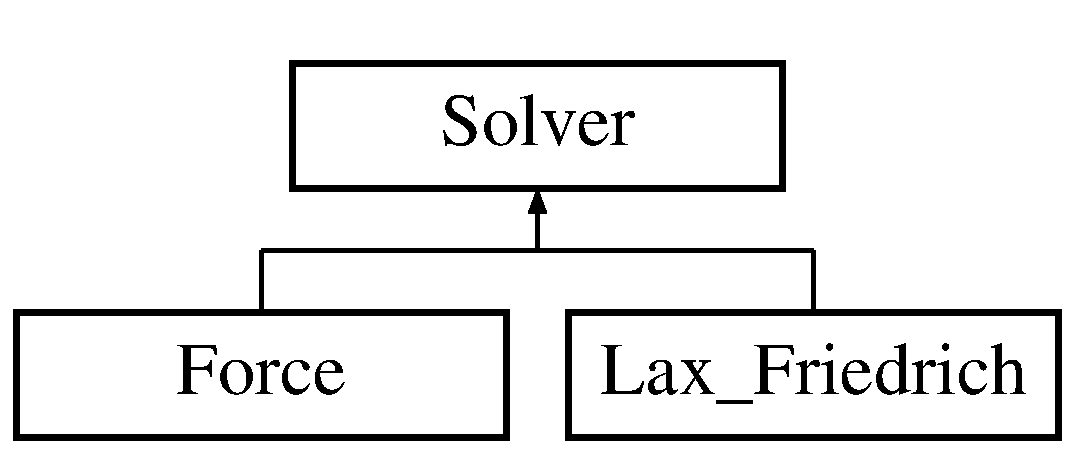
\includegraphics[height=2.000000cm]{classSolver}
\end{center}
\end{figure}
\subsection*{Public Member Functions}
\begin{DoxyCompactItemize}
\item 
\hyperlink{classSolver_a0075747c547c2da8911f2c95bdadaed4}{Solver} (string solver\-\_\-name, \hyperlink{classConstants}{Constants} $\ast$\hyperlink{classSolver_af8791d3a5042e7be5980ae3247cb60de}{constants}, \hyperlink{classComputation}{Computation} $\ast$\hyperlink{classSolver_a158efd10f04099b8be28561f990b646a}{computation}, \hyperlink{classGrid}{Grid} $\ast$\hyperlink{classSolver_a147ba19192faf8f24dadfc569f3d403f}{grid})
\item 
virtual void \hyperlink{classSolver_ab0c03d26d92272de997fa6984a2a86de}{calc\-\_\-method\-\_\-flux} (double dt, int dir)=0
\end{DoxyCompactItemize}
\subsection*{Public Attributes}
\begin{DoxyCompactItemize}
\item 
\hyperlink{classConstants}{Constants} $\ast$ \hyperlink{classSolver_af8791d3a5042e7be5980ae3247cb60de}{constants}
\item 
\hyperlink{classGrid}{Grid} $\ast$ \hyperlink{classSolver_a147ba19192faf8f24dadfc569f3d403f}{grid}
\item 
\hyperlink{classComputation}{Computation} $\ast$ \hyperlink{classSolver_a158efd10f04099b8be28561f990b646a}{computation}
\item 
\hypertarget{classSolver_a75135e4bd38563a60b6682856946b595}{string {\bfseries name}}\label{classSolver_a75135e4bd38563a60b6682856946b595}

\item 
int \hyperlink{classSolver_a9f81101cc1872e3da6b2f20fb678fa02}{dimension}
\item 
double \hyperlink{classSolver_a52a573400ef79611f2b7cf28e0a101ac}{dx}
\item 
double \hyperlink{classSolver_a716c9ccbc57382159d803e8fe7e9874b}{dy}
\item 
int $\ast$ \hyperlink{classSolver_accc6d00868567cda6fc234b3c1934a13}{size\-\_\-total}
\item 
int $\ast$ \hyperlink{classSolver_ab954613f6a40bbcbcbc7c04469f36db5}{size\-\_\-m1}
\end{DoxyCompactItemize}


\subsection{Detailed Description}
Abstrakte Klasse für sämtliche Methoden zur Lösung von Differential Gleichungen 

\subsection{Constructor \& Destructor Documentation}
\hypertarget{classSolver_a0075747c547c2da8911f2c95bdadaed4}{\index{Solver@{Solver}!Solver@{Solver}}
\index{Solver@{Solver}!Solver@{Solver}}
\subsubsection[{Solver}]{\setlength{\rightskip}{0pt plus 5cm}Solver\-::\-Solver (
\begin{DoxyParamCaption}
\item[{string}]{solver\-\_\-name, }
\item[{{\bf Constants} $\ast$}]{constants, }
\item[{{\bf Computation} $\ast$}]{computation, }
\item[{{\bf Grid} $\ast$}]{grid}
\end{DoxyParamCaption}
)}}\label{classSolver_a0075747c547c2da8911f2c95bdadaed4}
Konstruktor. 
\begin{DoxyParams}{Parameters}
{\em dim} & Setzt Dimension für die Berechnung. \\
\hline
{\em ordn} & Ordnung der numerischen Methode. \\
\hline
{\em cells} & Anzahl der Zellen. \\
\hline
{\em method} & Name der Methode für unterscheidung bei Output. \\
\hline
\end{DoxyParams}


\subsection{Member Function Documentation}
\hypertarget{classSolver_ab0c03d26d92272de997fa6984a2a86de}{\index{Solver@{Solver}!calc\-\_\-method\-\_\-flux@{calc\-\_\-method\-\_\-flux}}
\index{calc\-\_\-method\-\_\-flux@{calc\-\_\-method\-\_\-flux}!Solver@{Solver}}
\subsubsection[{calc\-\_\-method\-\_\-flux}]{\setlength{\rightskip}{0pt plus 5cm}virtual void Solver\-::calc\-\_\-method\-\_\-flux (
\begin{DoxyParamCaption}
\item[{double}]{dt, }
\item[{int}]{dir}
\end{DoxyParamCaption}
)\hspace{0.3cm}{\ttfamily [pure virtual]}}}\label{classSolver_ab0c03d26d92272de997fa6984a2a86de}
Abstrakte Methode zur berechnung des Flusses der jeweiligen numerischen Methode. \begin{DoxyReturn}{Returns}
Matrix der Flüsse (1\-D) 
\end{DoxyReturn}


Implemented in \hyperlink{classLax__Friedrich_a77ace0aa368e5b04263b23a69d2b3fe7}{Lax\-\_\-\-Friedrich}, and \hyperlink{classForce_a6c395b2d375796332c6d688760c79dc4}{Force}.



\subsection{Member Data Documentation}
\hypertarget{classSolver_a158efd10f04099b8be28561f990b646a}{\index{Solver@{Solver}!computation@{computation}}
\index{computation@{computation}!Solver@{Solver}}
\subsubsection[{computation}]{\setlength{\rightskip}{0pt plus 5cm}{\bf Computation}$\ast$ Solver\-::computation}}\label{classSolver_a158efd10f04099b8be28561f990b646a}
Gleichungssystem Objekt. \begin{DoxySeeAlso}{See Also}
Gleichungssystem 
\end{DoxySeeAlso}
\hypertarget{classSolver_af8791d3a5042e7be5980ae3247cb60de}{\index{Solver@{Solver}!constants@{constants}}
\index{constants@{constants}!Solver@{Solver}}
\subsubsection[{constants}]{\setlength{\rightskip}{0pt plus 5cm}{\bf Constants}$\ast$ Solver\-::constants}}\label{classSolver_af8791d3a5042e7be5980ae3247cb60de}
\hyperlink{classKonstanten}{Konstanten} Objekt welches für die berechnungen benötigt wird. \begin{DoxySeeAlso}{See Also}
\hyperlink{classKonstanten}{Konstanten} 
\end{DoxySeeAlso}
\hypertarget{classSolver_a9f81101cc1872e3da6b2f20fb678fa02}{\index{Solver@{Solver}!dimension@{dimension}}
\index{dimension@{dimension}!Solver@{Solver}}
\subsubsection[{dimension}]{\setlength{\rightskip}{0pt plus 5cm}int Solver\-::dimension}}\label{classSolver_a9f81101cc1872e3da6b2f20fb678fa02}
Dimension in der gerechnet wird. \hypertarget{classSolver_a52a573400ef79611f2b7cf28e0a101ac}{\index{Solver@{Solver}!dx@{dx}}
\index{dx@{dx}!Solver@{Solver}}
\subsubsection[{dx}]{\setlength{\rightskip}{0pt plus 5cm}double Solver\-::dx}}\label{classSolver_a52a573400ef79611f2b7cf28e0a101ac}
Delta x. \hypertarget{classSolver_a716c9ccbc57382159d803e8fe7e9874b}{\index{Solver@{Solver}!dy@{dy}}
\index{dy@{dy}!Solver@{Solver}}
\subsubsection[{dy}]{\setlength{\rightskip}{0pt plus 5cm}double Solver\-::dy}}\label{classSolver_a716c9ccbc57382159d803e8fe7e9874b}
Delta y für die 2. Dimension \hypertarget{classSolver_a147ba19192faf8f24dadfc569f3d403f}{\index{Solver@{Solver}!grid@{grid}}
\index{grid@{grid}!Solver@{Solver}}
\subsubsection[{grid}]{\setlength{\rightskip}{0pt plus 5cm}{\bf Grid}$\ast$ Solver\-::grid}}\label{classSolver_a147ba19192faf8f24dadfc569f3d403f}
Raster in den gerechnet wird. \begin{DoxySeeAlso}{See Also}
Raster 
\end{DoxySeeAlso}
\hypertarget{classSolver_ab954613f6a40bbcbcbc7c04469f36db5}{\index{Solver@{Solver}!size\-\_\-m1@{size\-\_\-m1}}
\index{size\-\_\-m1@{size\-\_\-m1}!Solver@{Solver}}
\subsubsection[{size\-\_\-m1}]{\setlength{\rightskip}{0pt plus 5cm}int$\ast$ Solver\-::size\-\_\-m1}}\label{classSolver_ab954613f6a40bbcbcbc7c04469f36db5}
Größe des Rasters für die Flussberechnung \hypertarget{classSolver_accc6d00868567cda6fc234b3c1934a13}{\index{Solver@{Solver}!size\-\_\-total@{size\-\_\-total}}
\index{size\-\_\-total@{size\-\_\-total}!Solver@{Solver}}
\subsubsection[{size\-\_\-total}]{\setlength{\rightskip}{0pt plus 5cm}int$\ast$ Solver\-::size\-\_\-total}}\label{classSolver_accc6d00868567cda6fc234b3c1934a13}
Größe des Rasters 

The documentation for this class was generated from the following files\-:\begin{DoxyCompactItemize}
\item 
solver.\-h\item 
solver.\-cpp\end{DoxyCompactItemize}

%--- End generated contents ---

% Index
\newpage
\phantomsection
\addcontentsline{toc}{part}{Index}
\printindex

\end{document}
